
\documentclass[aps, prd
, preprint
%, twocolumn
, nofootinbib 
%, notitlepage
%, superscriptaddress
]{revtex4-1}
\usepackage{graphicx}
\usepackage[caption=false]{subfig}
\usepackage{mathrsfs}
\usepackage{amsmath,amssymb}
\usepackage{bm}
\usepackage{braket}
\usepackage{listings}
\usepackage{cases}
\usepackage{comment}
\usepackage{soul}
\usepackage{cancel}
\usepackage{cases}
\usepackage[utf8]{inputenc}
\usepackage{url}
\usepackage{longtable}
\usepackage[normalem]{ulem}
\usepackage[colorlinks=true
,urlcolor=blue
,anchorcolor=blue
,citecolor=blue
,filecolor=blue
,linkcolor=blue
,menucolor=blue
,pagecolor=blue
,linktocpage=true
,pdfproducer=medialab
,pdfa=true
]{hyperref}

%\usepackage{mathpazo}
%\usepackage[no-math]{fontspec}
%\setmainfont{Palatino}
%\setsansfont{Optima}

\newcommand{\dif}[2]{\frac{\mathrm{d} #1}{\mathrm{d} #2}}
\newcommand{\pdif}[2]{\frac{\partial #1}{\partial #2}}
\newcommand{\var}[2]{\frac{\delta #1}{\delta #2}}
\newcommand{\dd}{\mathrm{d}}
\newcommand{\DD}{\mathscr{D}}
\newcommand{\ee}{\mathrm{e}}
\newcommand{\diag}{\mathrm{diag}}
\newcommand{\sgn}{\mathrm{sgn}}
\newcommand{\Mpl}{M_\text{Pl}}
\newcommand{\ns}{n_{{}_\mathrm{S}}}
\newcommand{\calP}{\mathcal{P}}
\newcommand{\cs}{c_{{}_\mathrm{S}}}
\newcommand{\IR}{\text{IR}}
\newcommand{\UV}{\text{UV}}
\renewcommand{\Re}{\mathrm{Re}}
\renewcommand{\Im}{\mathrm{Im}}
\newcommand{\dk}{\frac{\dd^3k}{(2\pi)^3}}
\newcommand{\bbalpha}{{\alpha\!\!\!\alpha}}
\newcommand{\dps}{\displaystyle}
\newcommand{\calJ}{\mathcal{J}}
\newcommand{\scrJ}{\mathscr{J}}
\newcommand{\calN}{\mathcal{N}}
\newcommand{\scrD}{\mathscr{D}}
\newcommand{\SIA}{S_\text{IA}}
\newcommand{\calD}{\mathcal{D}}

\newcommand{\bae}[1]{\begin{align} #1 \end{align}}
\newcommand{\bce}[1]{\begin{cases} #1 \end{cases}}
\newcommand{\bfe}[4]{
\begin{figure} 
	\centering
	\includegraphics[#1]{#2}
	\caption{#3}
	\label{#4}
\end{figure}}
\newcommand{\bpme}[1]{\begin{pmatrix} #1 \end{pmatrix}}

\newcommand{\Red}[1]{\textcolor{red}{\sffamily #1}}
\newcommand{\Mag}[1]{\textcolor{magenta}{\sffamily #1}}
\newcommand{\Blue}[1]{\textcolor{blue}{\sffamily #1}}
\newcommand{\mathblue}[1]{\textcolor{blue}{#1}}



\begin{document}
\title{Langevin equations in the non-linear sigma model}
\date{\today}

%\author{Lucas Pinol}
%\email{pinol@iap.fr}

\author{Sébastien Renaux-Petel}
\email{renaux@iap.fr}

\author{Yuichiro Tada}
\email{tada@iap.fr}
\affiliation{Institut d’Astrophysique de Paris, UMR-7095 du CNRS, Université Pierre et Marie Curie, 98 bis bd Arago, 75014 Paris, France}
\affiliation{Sorbonne Universités, Institut Lagrange de Paris, 98 bis bd Arago, 75014 Paris, France}


\begin{abstract}
In these working notes, we derive the Langevin equations from the first principle action by integrating out the subhorizon modes.
Refs.: \cite{Morikawa:1989xz,Levasseur:2013ffa}.
\end{abstract}

\maketitle
\tableofcontents
%\vfill

%\newpage


\part{Lagrangian formalism}

\section{Canonical single field}

As a warming-up, let us start by the simplest example: the canonical single field case as
\bae{\label{eq: action of canonical single field}
	S=\int\dd^4x\sqrt{-g}\left[-\frac{1}{2}g^{\mu\nu}\partial_\mu\phi\partial_\nu\phi-V(\phi)\right].
}
Here the potential $V(\phi)$ is not necessarily quadratic and we consider a more generic function.
For a while we neglect the metric perturbations and assume that the metric $g_{\mu\nu}$ is given by the FLRW one:
\bae{
	g_{\mu\nu}=\diag(-1,a^2(t),a^2(t),a^2(t)).
}
In this case the action~(\ref{eq: action of canonical single field}) reads
\bae{
	S=\int\dd^4x\,a^3\left[\frac{1}{2}\dot{\phi}^2-\frac{1}{2a^2}\partial_i\phi\partial_i\phi-V(\phi)\right].
}
Now let us divide $\phi$ into the IR mode $\varphi$ and UV mode $Q$ as
\bae{
	\phi(x)&=\varphi(x)+Q(x), \\
	Q(x)&=\int\dk W\left(\frac{k}{\sigma aH}\right)\phi_\mathbf{k}(t)\ee^{i\mathbf{k}\cdot\mathbf{x}},
}
where $W(z)$ is a certain window function taking the subhorizon modes $k\gtrsim\sigma aH$ 
with a small positive parameter $\sigma$. Hereafter we will basically consider the step window function $\theta(k-\sigma aH)$ for simplicity. 
Up to quadratic order in $Q$, the action reads
\bae{\label{eq: quadratic action in canonical single}
	S&=S^{(0)}+S^{(1)}+S^{(2)}+\mathcal{O}(Q^3), \\
	S^{(0)}&=S[\varphi]=\int\dd^4x\,a^3\left[\frac{1}{2}\dot{\varphi}^2-V(\varphi)\right], \\
	S^{(1)}&=\int\dd^4x\,QE(\varphi), \quad\quad S^{(2)}=\int\dd^4x\frac{1}{2}Q\Lambda Q,
}
with
\bae{
	E(\varphi)&=-a^3\left[\left(\partial_t^2+3H\partial_t\right)\varphi+V^\prime\right], \\
	\Lambda&=-a^3\left[\left(\partial_t^2+3H\partial_t-\frac{\nabla^2}{a^2}+V^{\prime\prime}\right)\right].
}
Here we neglected the gradient terms for the IR mode $\varphi$.
Note that at the classical level, the EoM for $\varphi$ and $Q$ are given by
\bae{
	E(\varphi)=0, \quad\quad \Lambda Q=0,
}
but due to the effect of the Hubble crossing of the UV mode, $\varphi$'s EoM will be modified by noise terms
as we will show.




\subsection{Effective action}

Now we want to calculate the expectation values of various quantities with the interactions described by 
the action~(\ref{eq: quadratic action in canonical single}).
Though the calculation of the scattering process, that is, the expectation value between the in- and out-vacuum is well-established,
what we want now is that between the in- and in-vacuum. In such a situation, one generally considers the problem after reducing it to
that of the scattering process.
In other words, one can interpret the in-in one as the scattering process on the closed time path from the in- to out- and then in-vacuum again.
The partition function is then calculated on the closed time path $C$ as
\bae{
	Z[J]=\mathcal{N}\int_C\mathscr{D}\phi\,\ee^{i\left(S+\int\dd^4xJ\phi\right)}
	=\mathcal{N}\left(\int_{C^+}\mathscr{D}\phi\,\ee^{i\left(S+\int\dd^4xJ\phi\right)}+\int_{C^-}\mathscr{D}\phi\,\ee^{i\left(S+\int\dd^4xJ\phi\right)}\right),
}
where $C^+$ and $C^-$ are the time paths from the in- to out-vacuum and from the out- to in-vacuum respectively.
$\mathcal{N}$ formally denotes the field independent normalization factor which does not necessarily take the same value
in differential equations.
If one expresses the field on $C^{+/-}$ as $\phi^{+/-}$, the partition function can be simplified to the standard 
scattering process with doubled d.o.f. as
\bae{
	Z[J^+,J^-]=\mathcal{N}\int_{t=-\infty\to+\infty}\mathscr{D}\phi^+\mathscr{D}\phi^-
	\exp\left[i\left\{S[\phi^+]-S[\phi^-]+\int\dd^4x\left(J^+\phi^+-J^-\phi^-\right)\right\}\right].
}
The negative sign for $S[\phi^-]$ comes from the inverted time flow.
Dividing fields and source terms into IR and UV modes, it reads
\bae{
	&Z[\mathcal{J}^\pm,\mathscr{J}^\pm]=\mathcal{N}\int\mathscr{D}\varphi^{\pm}\mathscr{D}Q^{\pm} 
	\exp\left[i\left\{S[\varphi^+]-S[\varphi^-]
	+\int\dd^4x\left(\mathcal{J}^+\varphi^+-\mathcal{J}^-\varphi^-\right)\right\}\right] \nonumber \\
	&\times\exp\left[i\int\dd^4x\,\left(Q^+E(\varphi^+)-Q^-E(\varphi^-)
	+\frac{1}{2}Q^+\tilde{\Lambda}(\varphi^+)Q^+-\frac{1}{2}Q^-\tilde{\Lambda}(\varphi^-)Q^-
	+\mathscr{J}^+Q^+-\mathscr{J}^-Q^-\right)\right].
}
Let us introduce a two-dimensional metric $\text{diag}(1,-1)$ for $+/-$ and the matrix derivative operator
\bae{
	\Lambda^a{}_b(x,y)=
	\bpme{
		\Lambda(\varphi^+(x)) & 0 \\
		0 & \Lambda(\varphi^-(x))
	}
	\delta^{(4)}(x-y).
}
Here indices $a$ and $b$ run over $+$ and $-$ and note that the time derivative in $\Lambda(\varphi(x))$ is w.r.t. $x^0$.
Suppressing the explicit expressions of the spacetime integrals,
the partition function can be simplified to
\bae{
	Z[\mathcal{J}^\pm,\mathscr{J}^\pm]=&\mathcal{N}\int\mathscr{D}\varphi^\pm
	\ee^{i\left(S[\varphi^+]-S[\varphi^-]+\mathcal{J}_a\varphi^a\right)}
	\int\mathscr{D}Q^\pm\exp\left[i\left(Q_{a}E^a+\frac{1}{2}Q_{a}\Lambda^a{}_bQ^{b}+\mathscr{J}_{a}Q^{a}\right)\right].
}
Since the $Q$ sector is quadratic, the free field part for $Q$ which does not depend on $\mathscr{J}$
can be easily renormalized into the normalization factor $\mathcal{N}$ by shifting the field as 
$Q^a\to Q^a+(\Lambda^{-1})^a{}_b(E^b+\mathscr{J}^b)$:
\bae{
	Z[\mathcal{J}^\pm,\mathscr{J}^\pm]=\mathcal{N}\int\mathscr{D}\varphi^\pm\ee^{i\left(S[\varphi^+]-S[\varphi^-]+\mathcal{J}_a\varphi^a\right)}
	\exp\left[-\frac{i}{2}(E_a+\mathscr{J}_a)(\Lambda^{-1})^a{}_b(E^b+\mathscr{J}^b)\right].
}
Finally here let us make a key assumption that\emph{the IR modes are well classicalized so that the integration w.r.t. $\varphi$ 
simply leads the replacement of $\varphi$ to the vev $\braket{\varphi}_\mathcal{J}$ 
under the existence of the source term $\mathcal{J}$}.
$\braket{\varphi}_\mathcal{J}$ should include the quantum effect by the subhorizon mode $Q$, and therefore 
its dynamics will be written by the Langevin equation what we want.
The partition function after the field integration can be given by
\bae{\label{eq: solved partition function}
	Z[\mathcal{J}^\pm,\mathscr{J}^\pm]\simeq\mathcal{N}\exp\left[i\left(S[\braket{\varphi^+}_\mathcal{J}]-S[\braket{\varphi^-}]_\mathcal{J}
	+\mathcal{J}_a\braket{\varphi^a}_\mathcal{J}-\frac{1}{2}(E_a+\mathscr{J}_a)(\Lambda^{-1})^a{}_b(E^a+\mathscr{J}^a)\right)\right].
}

Since now we obtained the explicit form of the partition function, any correlation function can be calculated simply by 
differentiating it w.r.t. $\mathcal{J}$ or $\mathscr{J}$. However for the dynamics of the field vev, the effective action $\Gamma$ is more useful.
Defining $iW$ by the exponent of $Z$ as
\bae{
	W[\mathcal{J}^\pm,\mathscr{J}^\pm]=S[\braket{\varphi^+}_\mathcal{J}]-S[\braket{\varphi^-}_\mathcal{J}]
	+\mathcal{J}_a\braket{\varphi^a}_\mathcal{J}-\frac{1}{2}(E_a+\mathscr{J}_a)(\Lambda^{-1})^a{}_b(E^b+\mathscr{J}^b),
}
the effective action is given by its Legendre transformation:
\bae{\label{eq: def of Gamma}
	\Gamma[\braket{\varphi^\pm},\braket{Q^\pm}]=W[\mathcal{J}^\pm,\mathscr{J}^\pm]-\mathcal{J}_a\braket{\varphi^a}-\mathscr{J}_a\braket{Q^a}.
}
Here the field vev and the source term are related by
\bae{\label{eq: Legendre relation}
	\braket{\varphi^a}=\frac{\delta W}{\delta\mathcal{J}_a}, \quad\quad \braket{Q^a}=\frac{\delta W}{\delta\mathscr{J}_a}.
}
While the IR part is already written in terms of $\braket{\varphi}$ due to the classicalization assumption,
one has to obtain the explicit solution of $\braket{Q}$ to eliminate the $\mathscr{J}$ dependence from Eq.~(\ref{eq: def of Gamma}).
The relation~(\ref{eq: Legendre relation}) gives rise to
\bae{
	\braket{Q^a}=-(\Lambda^{-1})^a{}_b(E^a+\mathscr{J}^a), \quad \Leftrightarrow \quad \mathscr{J}^a=-\Lambda^a{}_b\braket{Q^b}-E^a.
}
Therefore the explicit expression of the effective action is given by
\bae{
	\Gamma[\braket{\varphi^\pm},\braket{Q^\pm}]=S[\braket{\varphi^+}]-S[\braket{\varphi^-}]
	+\frac{1}{2}\braket{Q}_a\Lambda^a{}_b\braket{Q}^b+E_a\braket{Q}^a.
}
$\braket{Q}$ is solved as a stationary point of this effective action, that is,
\bae{
	\braket{Q^a}=-(\Lambda^{-1})^a{}_bE^b.
}
Substituting it back into the effective action, one finally obtains the effective action for $\braket{\varphi}$ as
\bae{
	\Gamma_\text{IR}[\braket{\varphi^\pm}]=S[\braket{\varphi^+}]-S[\braket{\varphi^-}]-\frac{1}{2}E_a(\Lambda^{-1})^a{}_bE^b,
}
and the last term $S_\text{IA}=-\frac{1}{2}E_a(\Lambda^{-1})^a{}_bE^b$ is called \emph{influence action}.
We will omit brackets hereafter for conciseness.





\subsection{Influence action}

The effect of the obtained influence action is still unclear. In this subsection let us go further on this term.
First note that the inverse of $Q$'s derivative operator is nothing but its propagator.
Indeed the time-ordered two point function of $Q$ can be obtained from the partition function~(\ref{eq: solved partition function}) as
\bae{
	\braket{T_CQ^a(x)Q_b(x^\prime)}=\left.\frac{1}{i}\frac{\delta}{\delta\mathscr{J}_a(x)}
	\frac{1}{i}\frac{\delta}{\delta\mathscr{J}^b(x^\prime)}Z\right|_{\mathcal{J}=\mathscr{J}=0}
	=i(\Lambda^{-1})^a{}_b(x,x^\prime).
}
Here we note that the normalization factor $\mathcal{N}$ is defined so that $\braket{1}=1$.
Also here time-ordering should be taken along the closed time path $C$, that is, the explicit order is given by
\bae{
	T_CQ^a(x)Q_b(x^\prime)=
	\bce{
		\displaystyle
		\theta(t-t^\prime)Q^a(x)Q_b(x^\prime)+\theta(t^\prime-t)Q_b(x^\prime)Q^a(x), & \text{($a=+$, $b=+$),} \\
		\displaystyle
		Q_b(x^\prime)Q^a(x), & \text{($a=+$, $b=-$),} \\
		\displaystyle
		Q^a(x)Q_b(x^\prime), & \text{($a=-$, $b=+$),} \\
		\displaystyle
		\theta(t^\prime-t)Q^a(x)Q_b(x^\prime)+\theta(t-t^\prime)Q_b(x^\prime)Q^a(x), & \text{($a=-$, $b=-$).}
	}
}
Expanding the field operator $\hat{Q}(x)$ as 
\bae{
	\hat{Q}(x)=\int\dk W\left(\frac{k}{\sigma aH}\right)\left[\phi_k(t)\hat{a}(\mathbf{k})\ee^{i\mathbf{k}\cdot\mathbf{x}}
	+\phi_k^*(t)\hat{a}^\dagger(\mathbf{k})\ee^{-i\mathbf{k}\cdot\mathbf{x}}\right],
}
with the annihilation-creation operators $\hat{a}(\mathbf{k})$ and $\hat{a}^\dagger(\mathbf{k})$ normalized by
\bae{
	[\hat{a}(\mathbf{k}),\hat{a}^\dagger(\mathbf{q})]=(2\pi)^3\delta^{(3)}(\mathbf{k}-\mathbf{q}),
}
the propagator can be written in terms of the mode function $\phi_k(t)$ as
\bae{
	&\braket{T_CQ^a(x)Q_b(x^\prime)}=\int\dk W\left(\frac{k}{\sigma aH|_t}\right)W\left(\frac{k}{\sigma aH|_{t^\prime}}\right) \nonumber \\
	&\times
	\bce{
		\displaystyle
		\theta(t-t^\prime)\phi_k^a(t)\phi_{k,b}^*(t^\prime)\ee^{i\mathbf{k}\cdot(\mathbf{x}-\mathbf{x}^\prime)}
		+\theta(t^\prime-t)\phi_{k,b}(t^\prime)\phi_k^{a*}(t)\ee^{i\mathbf{k}\cdot(\mathbf{x}^\prime-\mathbf{x})}, &
		\text{($a=+$, $b=+$)}, \\
		\displaystyle
		\phi_{k,b}(t^\prime)\phi_k^{a*}(t)\ee^{i\mathbf{k}\cdot(\mathbf{x}^\prime-\mathbf{x})}, &
		\text{($a=+$, $b=-$)}, \\
		\displaystyle
		\phi_k^a(t)\phi_{k,b}^*(t^\prime)\ee^{i\mathbf{k}\cdot(\mathbf{x}-\mathbf{x}^\prime)}, &
		\text{($a=-$, $b=+$)}, \\
		\displaystyle
		\theta(t^\prime-t)\phi_k^a(t)\phi_{k,b}^*(t^\prime)\ee^{i\mathbf{k}\cdot(\mathbf{x}-\mathbf{x}^\prime)}
		+\theta(t-t^\prime)\phi_{k,b}(t^\prime)\phi_k^{a*}(t)\ee^{i\mathbf{k}\cdot(\mathbf{x}^\prime-\mathbf{x})}, &
		\text{($a=-$, $b=-$)}.
	}
}
The mode function $\phi_k(t)$ is given by the solution of the subhorizon EoM:
\bae{
	\tilde{\Lambda}\phi_k=-a^3\left[\left(\partial_t^2+3H\partial_t+\frac{k^2}{a^2}+V^{\prime\prime}\right)\right]\phi_k=0,
}
and $+/-$ indices for them can be taken into account as $\phi_k^+=\phi_{k,+}=\phi_k^-=-\phi_{k,-}=\phi_k$.\footnote{Since the coefficients
$H$ and $V^{\prime\prime}$ in the EoM depend on the background IR mode $\varphi^\pm$,
the solutions $\phi_k^+$ and $\phi_k^-$ are generally different. However we will consider the IR EoM at $\varphi^+=\varphi^-$
and therefore these two solutions can be given by the same $\phi_k$.}
The explicit expression of the influence action then reads
\bae{
	S_\text{IA}=&-\frac{1}{2}E_a(\Lambda^{-1})^a{}_bE^b \nonumber \\
	=&\frac{i}{2}\int\dd^4x\dd^4x^\prime\int\dk a^3(t)\left[(\partial_t^2+3H\partial_t)\varphi_a(x)+V^\prime_a(x)\right]
	W\left(\frac{k}{\sigma aH|_t}\right) \nonumber \\
	&\times\bpme{
		\begin{array}{c}
			\theta(t-t^\prime)\phi_k(t)\phi_{k}^*(t^\prime)\ee^{i\mathbf{k}\cdot(\mathbf{x}-\mathbf{x}^\prime)} \\
			+\theta(t^\prime-t)\phi_{k}(t^\prime)\phi_k^{*}(t)\ee^{i\mathbf{k}\cdot(\mathbf{x}^\prime-\mathbf{x})}
		\end{array} &
		-\phi_{k}(t^\prime)\phi_k^{*}(t)\ee^{i\mathbf{k}\cdot(\mathbf{x}^\prime-\mathbf{x})} \\
		\phi_k(t)\phi_{k}^*(t^\prime)\ee^{i\mathbf{k}\cdot(\mathbf{x}-\mathbf{x}^\prime)} &
		\begin{array}{c}
			-\theta(t^\prime-t)\phi_k(t)\phi_{k}^*(t^\prime)\ee^{i\mathbf{k}\cdot(\mathbf{x}-\mathbf{x}^\prime)} \\
			-\theta(t-t^\prime)\phi_{k}(t^\prime)\phi_k^{*}(t)\ee^{i\mathbf{k}\cdot(\mathbf{x}^\prime-\mathbf{x})}
		\end{array}
	}{}^a{}_b \nonumber \\
	&\times W\left(\frac{k}{\sigma aH|_{t^\prime}}\right)
	\left[(\partial_{t^\prime}^2+3H\partial_{t^\prime})\varphi^b(x^\prime)+V^{\prime b}(x^\prime)\right]a^3(t^\prime).
}

\bigskip
Here let us mention the orthogonality between the IR and UV modes.
If the window function is taken to satisfy $W^2(z)=W(z)$ (e.g. the step function does),
the IR and UV modes are orthogonal to each other as
\bae{
	\int\dd^4x\varphi(x)Q(x)&=\int\dd^4x\int\frac{\dd^3k\dd^3k^\prime}{(2\pi)^6}\left(1-W\left(\frac{k}{\sigma aH}\right)\right)
	W\left(\frac{k^\prime}{\sigma aH}\right)\phi_\mathbf{k}\phi_{\mathbf{k}^\prime}\ee^{i(\mathbf{k}+\mathbf{k}^\prime)\cdot\mathbf{x}} \nonumber \\
	&=\int\dk\left(W\left(\frac{k}{\sigma aH}\right)-W^2\left(\frac{k}{\sigma aH}\right)\right)\phi_\mathbf{k}\phi_{-\mathbf{k}}=0.
}
On the other hand non-linear functions of $\varphi$ are not necessarily orthogonal to the UV mode due to the convolution.
For example 
\bae{
	&\int\dd^4x\varphi^2(x)Q(x) \nonumber \\
	&\quad=\int\frac{\dd^3k\dd^3k^\prime}{(2\pi)^6}\left(1-W\left(\frac{k}{\sigma aH}\right)\right)
	\left(1-W\left(\frac{k^\prime}{\sigma aH}\right)\right)W\left(\frac{|\mathbf{k}+\mathbf{k}^\prime|}{\sigma aH}\right)
	\phi_\mathbf{k}\phi_{\mathbf{k}^\prime}\phi_{-\mathbf{k}-\mathbf{k}^\prime},
}
and the integrand has non-zero contribution. 
However practically we will neglect the convolution effect and consider any quantity as it is re-coarse-grained.
That is, any function $f(\varphi)$ is replaced by its average over the Hubble scale:
\bae{
	f(\varphi(x))\to\int\dk\left(1-W\left(\frac{k}{\sigma aH}\right)\right)f_\mathbf{k}\ee^{i\mathbf{k}\cdot\mathbf{x}}.
}
After this replacement, the IR function is orthogonal to the UV mode.

Meanwhile if there is a time derivative, the IR mode is not orthogonal to the UV mode even after this re-coarse-graining.
For example
\bae{
	\int\dd^4x\dot{\varphi}(x)Q(x)&=-\int\dd^4x\varphi(x)\dot{Q}(x)=\int\dk\left(1-W\left(\frac{k}{\sigma aH}\right)\right)\phi_\mathbf{k}
	\partial_t\left(W\left(\frac{k}{\sigma aH}\right)\phi_{-\mathbf{k}}\right) \nonumber \\
	&=\int\dk\left(1-W\left(\frac{k}{\sigma aH}\right)\right)\phi_\mathbf{k}
	\dot{W}\left(\frac{k}{\sigma aH}\right)\phi_{-\mathbf{k}}.
}
Thanks to the time derivative of $W$, it does not vanish even though it is already coarse-grained as it includes $1-W(k/\sigma aH)$ factor.
Indeed such a term shows the effect of the Hubble crossing of the UV mode.
In summary, following the above consideration, we will keep only terms including time derivatives.

\bigskip
Now the influence action reads
\bae{
	S_\text{IA}=&\frac{i}{2}\int\dd^4x\dd^4x^\prime\int\dk a^3(t)\left[(\partial_t^2+3H\partial_t)\varphi_a(x)\right]
	W\left(\frac{k}{\sigma aH|_t}\right) \nonumber \\
	&\times\bpme{
		\begin{array}{c}
			\theta(t-t^\prime)\phi_k(t)\phi_{k}^*(t^\prime)\ee^{i\mathbf{k}\cdot(\mathbf{x}-\mathbf{x}^\prime)} \\
			+\theta(t^\prime-t)\phi_{k}(t^\prime)\phi_k^{*}(t)\ee^{i\mathbf{k}\cdot(\mathbf{x}^\prime-\mathbf{x})}
		\end{array} &
		-\phi_{k}(t^\prime)\phi_k^{*}(t)\ee^{i\mathbf{k}\cdot(\mathbf{x}^\prime-\mathbf{x})} \\
		\phi_k(t)\phi_{k}^*(t^\prime)\ee^{i\mathbf{k}\cdot(\mathbf{x}-\mathbf{x}^\prime)} &
		\begin{array}{c}
			-\theta(t^\prime-t)\phi_k(t)\phi_{k}^*(t^\prime)\ee^{i\mathbf{k}\cdot(\mathbf{x}-\mathbf{x}^\prime)} \\
			-\theta(t-t^\prime)\phi_{k}(t^\prime)\phi_k^{*}(t)\ee^{i\mathbf{k}\cdot(\mathbf{x}^\prime-\mathbf{x})}
		\end{array}
	}{}^a{}_b \nonumber \\
	&\times W\left(\frac{k}{\sigma aH|_{t^\prime}}\right)
	\left[(\partial_{t^\prime}^2+3H\partial_{t^\prime})\varphi^b(x^\prime)\right]a^3(t^\prime).
}
Integrating by parts and dropping terms without the time derivative of $W$, one obtains
\bae{
	S_\text{IA}=&\frac{i}{2}\int\dd^4x\dd^4x^\prime\int\dk\varphi_a(x)a^3(t)[\ddot{W}_t+3H\dot{W}_t+2\dot{W}_t\partial_t] \nonumber \\
	&\times\bpme{
		\begin{array}{c}
			\theta(t-t^\prime)\phi_k(t)\phi_{k}^*(t^\prime)\ee^{i\mathbf{k}\cdot(\mathbf{x}-\mathbf{x}^\prime)} \\
			+\theta(t^\prime-t)\phi_{k}(t^\prime)\phi_k^{*}(t)\ee^{i\mathbf{k}\cdot(\mathbf{x}^\prime-\mathbf{x})}
		\end{array} &
		-\phi_{k}(t^\prime)\phi_k^{*}(t)\ee^{i\mathbf{k}\cdot(\mathbf{x}^\prime-\mathbf{x})} \\
		\phi_k(t)\phi_{k}^*(t^\prime)\ee^{i\mathbf{k}\cdot(\mathbf{x}-\mathbf{x}^\prime)} &
		\begin{array}{c}
			-\theta(t^\prime-t)\phi_k(t)\phi_{k}^*(t^\prime)\ee^{i\mathbf{k}\cdot(\mathbf{x}-\mathbf{x}^\prime)} \\
			-\theta(t-t^\prime)\phi_{k}(t^\prime)\phi_k^{*}(t)\ee^{i\mathbf{k}\cdot(\mathbf{x}^\prime-\mathbf{x})}
		\end{array}
	}{}^a{}_b \nonumber \\
	&\times[\ddot{W}_{t^\prime}+3H\dot{W}_{t^\prime}+2\overleftarrow{\partial_{t^\prime}}\dot{W}_{t^\prime}]a^3(t^\prime)\varphi^b(x^\prime),
}
where 
\bae{
	W_t=W\left(\frac{k}{\sigma aH|_t}\right), \quad\quad W_{t^\prime}=W\left(\frac{k}{\sigma aH|_{t^\prime}}\right).
}
Then we move to the useful Keldysh $(\bar{\varphi},\varphi^\Delta)$ basis defined by
\bae{
	\bpme{
		\bar{\varphi} \\
		\varphi^\Delta
	}=\bpme{
		1/2 & 1/2 \\
		1 & -1
	}\bpme{
		\varphi^+ \\
		\varphi^-
	}, \quad \Leftrightarrow \quad
	\bpme{
		\varphi^+ \\
		\varphi^-
	}=\bpme{
		1& 1/2 \\
		1 & -1/2
	}\bpme{
		\bar{\varphi} \\
		\varphi^\Delta
	}.
}
In this basis, the influence action can be written as (\Blue{wrong})
\bae{
	S_\text{IA}=&\frac{i}{2}\int\dd^4x\dd^4x^\prime\varphi^\Delta(x)\Re[\Pi(x,x^\prime)]\varphi^\Delta(x^\prime) \nonumber \\
	&-\int\dd^4x\dd^4x^\prime[\theta(t-t^\prime)-\theta(t^\prime-t)]\varphi^\Delta(x)\Im[\Pi(x,x^\prime)]\bar{\varphi}(x^\prime),
}
where
\bae{
	\Pi(x,x^\prime)=\int\dk\ee^{i\mathbf{k}\cdot(\mathbf{x}-\mathbf{x}^\prime)}P\phi_k(t)P\phi^*_k(t^\prime),
}
with the operator
\bae{
	P=a^3\left[\ddot{W}_t+3H\dot{W}_t+2\dot{W}_t\partial_t\right].
}



\subsection{Fluctuation}

Let us first concentrate on the imaginary part of the influence action which gives rise to the noise term.
After integration by parts to avoid the second time derivative of $W$, it reads
\bae{
	\Im[S_\text{IA}]=&\frac{1}{2}\Re\left[\int\dd^4x\dd^4x^\prime\int\dk\ee^{i\mathbf{k}\cdot(\mathbf{x}-\mathbf{x}^\prime)} 
	a^3(t)a^3(t^\prime)\right. \nonumber \\
	&\left.\times\left(-\dot{\varphi}^\Delta(x)\dot{W}_t\phi_k(t)+\varphi^\Delta(x)\dot{W}_t\dot{\phi}_k(t)\right)
	\left(-\dot{\varphi}^\Delta(x^\prime)\dot{W}_{t^\prime}\phi_k^*(t^\prime)
	+\varphi^\Delta(x^\prime)\dot{W}_{t^\prime}\dot{\phi}_k^*(t^\prime)\right)\right],
}
where
\bae{
	\dot{W}_t=\dot{\theta}(k-\sigma aH|_t)=-\sigma aH^2(1-\epsilon_H)|_t\delta(k-\sigma aH|_t).
}
Now the integrals include two delta function as $\delta(k-\sigma aH|_t)\delta(k-\sigma aH|_{t^\prime})$ which
can be rewritten as 
$\delta(k-\sigma aH|_t)\delta(\sigma aH|_t-\sigma aH|_{t^\prime})=[\sigma aH^2(1-\epsilon_H)]^{-1}\delta(k-\sigma aH|_t)\delta(t-t^\prime)$.
Therefore one can assume $t=t^\prime$ and $k=\sigma aH$ in the integrals.
Also we introduce the $q$-parameter by
\bae{
	q(\sigma)=\left.\frac{\dot{\phi}_k}{\phi_k}\right|_{k=\sigma aH}.
}
Then one obtains
\bae{
	\Im[S_\text{IA}]=&\frac{1}{2}\Re\left[\int\dd^4x\dd^4x^\prime\int\dk\ee^{i\mathbf{k}\cdot(\mathbf{x}-\mathbf{x}^\prime)}
	a^6\dot{W}_t\dot{W}_{t^\prime}|\phi_k|^2_{k=\sigma aH} \right. \nonumber \\
	&\left.\times\left(\dot{\varphi}^\Delta(x)\dot{\varphi}^\Delta(x^\prime)-q\varphi^\Delta(x)\dot{\varphi}^\Delta(x^\prime)
	-q^*\dot{\varphi}^\Delta(x)\varphi^\Delta(x^\prime)+|q|^2\varphi^\Delta(x)\varphi^\Delta(x^\prime)\right)\right].
}
It can be much simplified in the basis of
\bae{
	\mathcal{Q}(x)=a^3(t)[\dot{\varphi}^\Delta(x)-q\varphi^\Delta(x)],
}
as
\bae{
	\Im[S_\text{IA}]=\frac{1}{2}\int\dd^4x\dd^4x^\prime\Re\left[\mathcal{Q}(x)\mathcal{A}(x,x^\prime)Q^*(x^\prime)\right],
}
where
\bae{
	\bce{
		\displaystyle
		\mathcal{A}(x,x^\prime)=\int\dk\ee^{i\mathbf{k}\cdot(\mathbf{x}-\mathbf{x}^\prime)}\dot{W}_t\dot{W}_{t^\prime}|\phi_k|^2_{k=\sigma aH}
		=H(1-\epsilon_H)\calP_\phi(\sigma aH)\frac{\sin(\sigma aH|\mathbf{x}-\mathbf{x}^\prime|)}{\sigma aH|\mathbf{x}-\mathbf{x}^\prime|}
		\delta(t-t^\prime), \\[10pt]
		\displaystyle
		\calP_\phi(k)=\frac{k^3}{2\pi^2}|\phi_k|^2.
	}
}

Now how should the imaginary part of the effective action be interpreted?
In the Keldysh basis, $\bar{\varphi}$ represents the classical trajectory and $\varphi^\Delta$ denotes the fluctuation from this trajectory.
Therefore the EoM for the classical trajectory is given by the variation of the effective action $\Gamma_\text{IR}$ w.r.t. $\varphi^\Delta$
at $\varphi^\Delta=0$, that is, $\delta\Gamma_\text{IR}/\delta\varphi^\Delta|_{\varphi^\Delta=0}=0$.
However if one directly varies $\Im[S_\text{IA}]$ at $\varphi^\Delta=0$, it vanished because $\Im[S_\text{IA}]$ is quadratic w.r.t. $\delta\varphi^\Delta$.
Does it mean that $\Im[S_\text{IA}]$ is meaningless?
In fact, to take account of the true contribution of $\Im[S_\text{IA}]$,
one has to introduce auxiliary fields $\xi^\text{R}$ and $\xi^\text{I}$ as
\bae{
	&\ee^{iS_\text{IA}}\propto\ee^{-\Im[S_\text{IA}]}=\exp\left[-\frac{1}{2}\int\dd^4x\dd^4x^\prime
	\Re\left[\mathcal{Q}(x)\mathcal{A}(x,x^\prime)Q^*(x^\prime)\right]\right] \nonumber \\
	&=\mathcal{N}\int\mathscr{D}\xi^{\text{R}/\text{I}}\exp\left[-\frac{1}{2}\int\dd^4x\dd^4x^\prime
	\left(\xi^\text{R}(x)\mathcal{A}^{-1}(x,x^\prime)\xi^\text{R}(x^\prime)+\xi^\text{I}(x)\mathcal{A}^{-1}(x,x^\prime)\xi^\text{I}(x^\prime)\right)\right.
	\nonumber \\
	&\quad\left.-i\int\dd^4x(\xi^\text{R}(x)\mathcal{Q}^\text{R}(x)+\xi^\text{I}(x)\mathcal{Q}^\text{I}(x))\right],
}
where $\mathcal{Q}^{\text{R}/\text{I}}$ represents the real/imaginary part of $\mathcal{Q}$ and we have used the Gaussian integral
\bae{
	&1=\mathcal{N}\int\mathscr{D}\xi^{\text{R}/\text{I}} \nonumber \\
	&\times\exp\left[-\frac{1}{2}\int\dd^4x\dd^4x^\prime
	\left(\xi^\text{R}(x)+i\int\dd^4y\mathcal{A}(x,y)\mathcal{Q}^\text{R}(y)\right)\mathcal{A}^{-1}(x,x^\prime)\left(\xi^\text{R}(x^\prime)
	+i\int\dd^4y^\prime\mathcal{A}(x^\prime,y^\prime)\mathcal{Q}^\text{R}(y^\prime)\right)\right. \nonumber \\
	&\left.-\frac{1}{2}\int\dd^4x\dd^4x^\prime
	\left(\xi^\text{I}(x)+i\int\dd^4y\mathcal{A}(x,y)\mathcal{Q}^\text{I}(y)\right)\mathcal{A}^{-1}(x,x^\prime)\left(\xi^\text{I}(x^\prime)
	+i\int\dd^4y^\prime\mathcal{A}(x^\prime,y^\prime)\mathcal{Q}^\text{I}(y^\prime)\right)\right]
}
with a normalization factor $\mathcal{N}$.\footnote{Strictly speaking, the noise amplitude $\mathcal{A}$ itself depends on the noise $\xi$
through its background dynamics dependence. Therefore the auxiliary fields $\xi$ are not completely Gaussian and this Gaussian integral
does not hold.
However the background dependence of $H$ or $\epsilon_H$ is suppressed in the slow-roll approximation.
Also in the single field case, $\phi$ is almost massless and the power spectrum of its fluctuation is given by $(H/2\pi)^2$ on the superhorizon scale.
Therefore its background dependence is slow-roll suppressed again. Then the noise $\xi$ can be regarded as almost Gaussian.
In the multi-field case and if one considers massive field, its power spectrum is not simply given by $(H/2\pi)^2$
and the non-Gaussianity of the corresponding noise will be large. In that case, however, the noise itself can be neglected since the noise amplitude
is strongly suppressed by its mass. Finally the tachyonic case does matter. The stochastic formalism can be justified only where both the 
tachyonic mass and its rate of change are not significant, compared to the Hubble parameter.}\vfill

Then one properly obtains the real effective action (neglecting the real part of $S_\text{IA}$ here):
\bae{
	S_\text{eff}=S[\varphi^+]-S[\varphi^-]-\int\dd^4x(\xi^\text{R}(x)\mathcal{Q}^\text{R}(x)+\xi^\text{I}(x)\mathcal{Q}^\text{I}(x)),
}
with the Gaussian auxiliary fields whose statistical properties can be summarized as
\bae{
	\bce{
		\displaystyle
		\braket{\xi^{\text{R}/\text{I}}(x)}=0 \\
		\braket{\xi^{\text{R}}(x)\xi^\text{I}(x^\prime)}=0 \\
		\braket{\xi^\text{R}(x)\xi^\text{R}(x^\prime)}=\braket{\xi^\text{I}(x)\xi^\text{I}(x^\prime)}=\mathcal{A}(x,x^\prime).
	}
}
They are nothing but the Gaussian noise. 
This effective action should be stationary against $\delta\varphi^\Delta$ at $\varphi^+=\varphi^-$, and this constraint gives
the Langevin equation as
\bae{
	\ddot{\bar{\varphi}}+3H\dot{\bar{\varphi}}+V^\prime=\dot\xi^\text{R}+3H\xi^\text{R}+q^\text{R}\xi^\text{R}+q^\text{I}\xi^\text{I},
}
where $q^{\text{R}/\text{I}}$ represents the real/imaginary part of $q$.
It can be decomposed into the EoM for $\bar{\varphi}$ and $\bar{\pi}$ as
\bae{
	\bce{
		\displaystyle
		\dot{\bar{\varphi}}=\bar{\pi}+\xi^\text{R}, \\
		\displaystyle
		\dot{\bar{\pi}}=-3H\bar{\pi}-V^\prime+q^\text{R}\xi^\text{R}+q^\text{I}\xi^\text{I}.
	}
}
Then the Morikawa's result is recovered.




\subsection{Dissipation}

Coming soon...





\section{Non-canonical single field}

In this section we then consider the case of single field, but whose kinetic term is non-canonical as
\bae{
	S=\int\dd^4x\sqrt{-g}\left[-\frac{1}{2}K(\phi)g^{\mu\nu}\partial_\mu\phi\partial_\nu\phi-V(\phi)\right].
}


\subsection{Canonical redefinition}

In the single field case, the problem can be reduced to the canonical kinetic one by the field redefinition
\bae{
	\psi(\phi)=\int^\phi\sqrt{K(\phi^\prime)}\dd\phi^\prime.
}
The action for this field $\psi$ is given by
\bae{
	S=\int\dd^4x\sqrt{-g}\left[-\frac{1}{2}g^{\mu\nu}\partial_\mu\psi\partial_\nu\psi-V(\phi(\psi))\right],
}
and the corresponding Langevin equation reads
\bae{
	\bce{
		\displaystyle
		\dot{\psi}=\pi+\xi^\text{R}, \\
		\displaystyle
		\dot{\pi}=-3H\pi-V^\prime\dif{\phi}{\psi}+q^\text{R}\xi^\text{R}+q^\text{I}\xi^\text{I}.
	}
}
With use of $\dd\psi/\dd\phi=\sqrt{K(\phi)}$, the Langevin equation for $\phi$ is given by
\bae{\label{eq: Langevin for non-canonical by field redefinition}
	\bce{
		\displaystyle
		\sqrt{K(\phi)}\dot{\phi}=\pi+\xi^\text{R}, \\
		\displaystyle
		\dot{\pi}=-3H\pi-\frac{V^\prime}{\sqrt{K(\phi)}}+q^\text{R}\xi^\text{R}+q^\text{I}\xi^\text{I}.
	}
}
The noise amplitude is given by the power spectrum of $\psi$:
\bae{
	\bce{
		\displaystyle
		\braket{\xi^\text{R}(x)}=\braket{\xi^\text{I}(x)}=\braket{\xi^\text{R}(x)\xi^\text{I}(x^\prime)}=0, \\
		\displaystyle
		\braket{\xi^\text{R}(x)\xi^\text{R}(x^\prime)}=\braket{\xi^\text{I}(x)\xi^\text{I}(x^\prime)}=H(1-\epsilon_H)\calP_\psi(\sigma aH)
		\frac{\sin(\sigma aH|\mathbf{x}-\mathbf{x}^\prime|)}{\sigma aH|\mathbf{x}-\mathbf{x}^\prime|}\delta(t-t^\prime),
	}
}
and the power of the canonical field $\psi$ is roughly $(H/2\pi)^2$ irrespectively of the transformation between $\phi$ and $\psi$.



\subsection{Without redefinition}

The redefinition approach can be applied only for the single field case because the field space curvature cannot be erased out by
the field redefinition in the multi-field case. 
Hence in this subsection, let us derive the Langevin equation without the field redefinition and compare the result with the previous
subsection's one~(\ref{eq: Langevin for non-canonical by field redefinition}).

Again we study the system by dividing the field into the IR and UV modes, but here we renormalize the UV mode as follows 
so that at least the UV mode is canonical and the corresponding noise is almost Gaussian:\footnote{Again there is a momentum coupling
(convolution) problem, but we neglect the mode coupling between IR functions and UV fields.}
\bae{\label{eq: UV renormalization}
	\phi(x)=\varphi(x)+Q(x)=\varphi(x)+\frac{1}{\sqrt{K(\varphi(x))}}\tilde{Q}(x).
}
In terms of the generic multi-field notation, the renormalization factor $1/\sqrt{K(\varphi)}$ corresponds with the vielbein.
Indeed in the single field case, the field space metric is $\gamma_{IJ}(\varphi)=K(\varphi)$ and
its inverse can be decomposed by the vielbein $e^I_\alpha$ as
\bae{
	\gamma^{IJ}=\frac{1}{K(\varphi)}, \quad\quad \gamma^{IJ}=\sum_\alpha e^I_\alpha e^J_\alpha, \quad\quad e^I_\alpha=\frac{1}{\sqrt{K(\varphi)}}.
}
The definition of $\tilde{Q}$~(\ref{eq: UV renormalization}) corresponds with
\bae{
	\phi^I(x)=\varphi^I(x)+e^I_\alpha\tilde{Q}_\alpha(x).
}
Note that the vielbein can be chosen to satisfy the parallel transportation condition as
\bae{
	D_te^I_\alpha=\partial_te^I_\alpha+\gamma^I_{JK}\dot{\varphi}^Je^K_\alpha=0,
}
and the definition $e^I_\alpha=1/\sqrt{K(\varphi)}$ satisfies this equation.
Reflecting the fact that $\tilde{Q}_\alpha$ has no longer the curved space indices $I,J,\cdots$,
this leads a following convenient relation.
\bae{
	D_tQ^I=e^I_\alpha\partial_t\tilde{Q}_\alpha.
}
Therefore at least in the linear perturbation theory, $\tilde{Q}$'s kinetic term is well canonicalized, and moreover
in the single-field case, there is no mass correction from the field space curvature since the Riemann tensor vanishes in one dimension.
Then the quadratic action can be given by quite simple expressions as\footnote{We here neglected the terms proportional to $E(\varphi)\tilde{Q}^2$
to obtain the expression of the quadratic action $S^{(2)}$. While $E(\varphi)$ does not vanish necessarily due to the noise term,
these terms are cubic order in the UV modes since the noise term itself comes from the UV modes. Therefore at the quadratic order,
one can drop them.}
\bae{
	S&\simeq S^{(0)}+S^{(1)}+S^{(2)}, \nonumber \\
	S^{(0)}&=S[\varphi], \\
	S^{(1)}&=\int\dd^4x\tilde{Q}(-a^3\sqrt{K})\left[\ddot{\varphi}+3H\dot{\varphi}+\frac{K^\prime}{2K}\dot{\varphi}^2+\frac{V^\prime}{K}\right]
	=\int\dd^4x\tilde{Q}E(\varphi), \\
	S^{(2)}&=\frac{1}{2}\int\dd^4x\tilde{Q}(-a^3)\left[\partial_t^2+3H\partial_t-\frac{\nabla^2}{a^2}+\frac{1}{K}\left(V^{\prime\prime}
	+\frac{K^\prime}{2K}V^\prime\right)\right]\tilde{Q}
	=\frac{1}{2}\int\dd^4x\tilde{Q}\Lambda\tilde{Q}.
}
Note that the mass term in $S^{(2)}$ corresponds with the covariant derivative of the potential as
\bae{
	\frac{1}{K}\left(V^{\prime\prime}+\frac{K^\prime}{2K}V^\prime\right)=e^I_\alpha e^J_\beta\left(V_{IJ}-\gamma^K_{IJ}V_K\right)
	=:e^I_\alpha e^J_\beta V_{I;J},
}
and it can be also written in terms of the canonical-field derivative
\bae{\label{eq: Vab}
	e^I_\alpha e^J_\beta V_{I;J}=\pdif{}{\varphi_\alpha}\pdif{}{\varphi_\beta}V=:V_{\alpha\beta},
}
where $\varphi_\alpha:=e^I_\alpha\varphi_I$.

The influence action is again given by
\bae{
	S_\text{IA}=-\frac{1}{2}E_a(\Lambda^{-1})^a{}_bE^b.
}
Keeping the terms including time derivatives, one obtains
\bae{
	S_\text{IA}=&\frac{i}{2}\int\dd^4x\dd^4x^\prime\int\dk a^3(t)\sqrt{K(\varphi(x))}
	\left[\ddot{\varphi}(x)+3H\dot{\varphi}(x)+\frac{K^\prime}{2K}\dot{\varphi}^2(x)\right]_a
	W\left(\frac{k}{\sigma aH|_t}\right) \nonumber \\
	&\times\bpme{
		\begin{array}{c}
			\theta(t-t^\prime)\tilde{\phi}_k(t)\tilde{\phi}_{k}^*(t^\prime)\ee^{i\mathbf{k}\cdot(\mathbf{x}-\mathbf{x}^\prime)} \\
			+\theta(t^\prime-t)\tilde{\phi}_{k}(t^\prime)\tilde{\phi}_k^{*}(t)\ee^{i\mathbf{k}\cdot(\mathbf{x}^\prime-\mathbf{x})}
		\end{array} &
		-\tilde{\phi}_{k}(t^\prime)\tilde{\phi}_k^{*}(t)\ee^{i\mathbf{k}\cdot(\mathbf{x}^\prime-\mathbf{x})} \\
		\tilde{\phi}_k(t)\tilde{\phi}_{k}^*(t^\prime)\ee^{i\mathbf{k}\cdot(\mathbf{x}-\mathbf{x}^\prime)} &
		\begin{array}{c}
			-\theta(t^\prime-t)\tilde{\phi}_k(t)\tilde{\phi}_{k}^*(t^\prime)\ee^{i\mathbf{k}\cdot(\mathbf{x}-\mathbf{x}^\prime)} \\
			-\theta(t-t^\prime)\tilde{\phi}_{k}(t^\prime)\tilde{\phi}_k^{*}(t)\ee^{i\mathbf{k}\cdot(\mathbf{x}^\prime-\mathbf{x})}
		\end{array}
	}{}^a{}_b \nonumber \\
	&\times W\left(\frac{k}{\sigma aH|_{t^\prime}}\right)
	\left.\left[\ddot{\varphi}(x^\prime)+3H\dot{\varphi}(x^\prime)+\frac{K^\prime}{2K}\dot{\varphi}^2(x^\prime)\right]
	\sqrt{K(\varphi(x^\prime))}\right|^ba^3(t^\prime).
}
After once integration by parts, it is much simplified as
\bae{
	S_\text{IA}=&\frac{i}{2}\int\dd^4x\dd^4x^\prime\int\dk a^3(t)\left.\sqrt{K(\varphi(x))}\dot{\varphi}(x)\right|_a\overrightarrow{\partial}_t
	W\left(\frac{k}{\sigma aH|_t}\right) \nonumber \\
	&\times\bpme{
		\begin{array}{c}
			\theta(t-t^\prime)\tilde{\phi}_k(t)\tilde{\phi}_{k}^*(t^\prime)\ee^{i\mathbf{k}\cdot(\mathbf{x}-\mathbf{x}^\prime)} \\
			+\theta(t^\prime-t)\tilde{\phi}_{k}(t^\prime)\tilde{\phi}_k^{*}(t)\ee^{i\mathbf{k}\cdot(\mathbf{x}^\prime-\mathbf{x})}
		\end{array} &
		-\tilde{\phi}_{k}(t^\prime)\tilde{\phi}_k^{*}(t)\ee^{i\mathbf{k}\cdot(\mathbf{x}^\prime-\mathbf{x})} \\
		\tilde{\phi}_k(t)\tilde{\phi}_{k}^*(t^\prime)\ee^{i\mathbf{k}\cdot(\mathbf{x}-\mathbf{x}^\prime)} &
		\begin{array}{c}
			-\theta(t^\prime-t)\tilde{\phi}_k(t)\tilde{\phi}_{k}^*(t^\prime)\ee^{i\mathbf{k}\cdot(\mathbf{x}-\mathbf{x}^\prime)} \\
			-\theta(t-t^\prime)\tilde{\phi}_{k}(t^\prime)\tilde{\phi}_k^{*}(t)\ee^{i\mathbf{k}\cdot(\mathbf{x}^\prime-\mathbf{x})}
		\end{array}
	}{}^a{}_b \nonumber \\
	&\times W\left(\frac{k}{\sigma aH|_{t^\prime}}\right)\overleftarrow{\partial}_{t^\prime}
	\left.\dot{\varphi}(x^\prime)
	\sqrt{K(\varphi(x^\prime))}\right|^ba^3(t^\prime).
}
One more integration by parts gives rise to
\bae{
	S_\text{IA}=&\frac{i}{2}\int\dd^4x\dd^4x^\prime\int\dk a^3(t)\sqrt{K(\varphi(x))}
	\left[\varphi(x)\partial_t+3H\varphi(x)+\frac{K^\prime}{2K}\dot{\varphi}\varphi(x)\right]_a\overrightarrow{\partial}_t
	W\left(\frac{k}{\sigma aH|_t}\right) \nonumber \\
	&\times\bpme{
		\begin{array}{c}
			\theta(t-t^\prime)\tilde{\phi}_k(t)\tilde{\phi}_{k}^*(t^\prime)\ee^{i\mathbf{k}\cdot(\mathbf{x}-\mathbf{x}^\prime)} \\
			+\theta(t^\prime-t)\tilde{\phi}_{k}(t^\prime)\tilde{\phi}_k^{*}(t)\ee^{i\mathbf{k}\cdot(\mathbf{x}^\prime-\mathbf{x})}
		\end{array} &
		-\tilde{\phi}_{k}(t^\prime)\tilde{\phi}_k^{*}(t)\ee^{i\mathbf{k}\cdot(\mathbf{x}^\prime-\mathbf{x})} \\
		\tilde{\phi}_k(t)\tilde{\phi}_{k}^*(t^\prime)\ee^{i\mathbf{k}\cdot(\mathbf{x}-\mathbf{x}^\prime)} &
		\begin{array}{c}
			-\theta(t^\prime-t)\tilde{\phi}_k(t)\tilde{\phi}_{k}^*(t^\prime)\ee^{i\mathbf{k}\cdot(\mathbf{x}-\mathbf{x}^\prime)} \\
			-\theta(t-t^\prime)\tilde{\phi}_{k}(t^\prime)\tilde{\phi}_k^{*}(t)\ee^{i\mathbf{k}\cdot(\mathbf{x}^\prime-\mathbf{x})}
		\end{array}
	}{}^a{}_b \nonumber \\
	&\times W\left(\frac{k}{\sigma aH|_{t^\prime}}\right)\overleftarrow{\partial}_{t^\prime}
	\left.\left[\overleftarrow{\partial}_{t^\prime}\varphi(x^\prime)+3H\varphi(x^\prime)+\frac{K^\prime}{2K}\dot{\varphi}\varphi(x^\prime)\right]
	\sqrt{K(\varphi(x^\prime))}\right|^ba^3(t^\prime).
}
Re-integrating by parts to avoid the second time derivative of $W$ and dropping the terms which have neither $\dot{\varphi}$ nor $\dot{W}$,
one obtains
\bae{
	S_\text{IA}=&\frac{i}{2}\int\dd^4x\dd^4x^\prime\int\dk a^3(t)\sqrt{K(\varphi(x))}
	\left[-\dot{\varphi}(x)\dot{W}_t+\varphi(x)\dot{W}_t\partial_t+\frac{K^\prime}{2K}\dot{\varphi}\varphi(x)W_t\partial_t\right]_a \nonumber \\
	&\times\bpme{
		\begin{array}{c}
			\theta(t-t^\prime)\tilde{\phi}_k(t)\tilde{\phi}_{k}^*(t^\prime)\ee^{i\mathbf{k}\cdot(\mathbf{x}-\mathbf{x}^\prime)} \\
			+\theta(t^\prime-t)\tilde{\phi}_{k}(t^\prime)\tilde{\phi}_k^{*}(t)\ee^{i\mathbf{k}\cdot(\mathbf{x}^\prime-\mathbf{x})}
		\end{array} &
		-\tilde{\phi}_{k}(t^\prime)\tilde{\phi}_k^{*}(t)\ee^{i\mathbf{k}\cdot(\mathbf{x}^\prime-\mathbf{x})} \\
		\tilde{\phi}_k(t)\tilde{\phi}_{k}^*(t^\prime)\ee^{i\mathbf{k}\cdot(\mathbf{x}-\mathbf{x}^\prime)} &
		\begin{array}{c}
			-\theta(t^\prime-t)\tilde{\phi}_k(t)\tilde{\phi}_{k}^*(t^\prime)\ee^{i\mathbf{k}\cdot(\mathbf{x}-\mathbf{x}^\prime)} \\
			-\theta(t-t^\prime)\tilde{\phi}_{k}(t^\prime)\tilde{\phi}_k^{*}(t)\ee^{i\mathbf{k}\cdot(\mathbf{x}^\prime-\mathbf{x})}
		\end{array}
	}{}^a{}_b \nonumber \\
	&\times \left.\left[-\dot{\varphi}(x^\prime)\dot{W}_{t^\prime}+\overleftarrow{\partial}_{t^\prime}\varphi(x^\prime)\dot{W}_{t^\prime}
	+\overleftarrow{\partial}_{t^\prime}\frac{K^\prime}{2K}\dot{\varphi}\varphi(x^\prime)W_{t^\prime}\right]
	\sqrt{K(\varphi(x^\prime))}\right|^ba^3(t^\prime).
}
Finally noting that 
\bae{
	\frac{K^\prime}{2\sqrt{K}}\dot{\varphi}\varphi=\partial_t\int^\varphi\frac{K^\prime}{2\sqrt{K}}\varphi^\prime\dd\varphi^\prime,
}
its integration by parts and the drop of terms without $\dot{W}$ lead
\bae{
	S_\text{IA}=&\frac{i}{2}\int\dd^4x\dd^4x^\prime\int\dk a^3(t)
	\left[-\sqrt{K}\dot{\varphi}(x)\dot{W}_t+\sqrt{K}\varphi(x)\dot{W}_t\partial_t
	-\left(\int^{\varphi(x)}\frac{K^\prime}{2\sqrt{K}}\varphi^\prime\dd\varphi^\prime\right)\dot{W}_t\partial_t\right]_a \nonumber \\
	&\times\bpme{
		\begin{array}{c}
			\theta(t-t^\prime)\tilde{\phi}_k(t)\tilde{\phi}_{k}^*(t^\prime)\ee^{i\mathbf{k}\cdot(\mathbf{x}-\mathbf{x}^\prime)} \\
			+\theta(t^\prime-t)\tilde{\phi}_{k}(t^\prime)\tilde{\phi}_k^{*}(t)\ee^{i\mathbf{k}\cdot(\mathbf{x}^\prime-\mathbf{x})}
		\end{array} &
		-\tilde{\phi}_{k}(t^\prime)\tilde{\phi}_k^{*}(t)\ee^{i\mathbf{k}\cdot(\mathbf{x}^\prime-\mathbf{x})} \\
		\tilde{\phi}_k(t)\tilde{\phi}_{k}^*(t^\prime)\ee^{i\mathbf{k}\cdot(\mathbf{x}-\mathbf{x}^\prime)} &
		\begin{array}{c}
			-\theta(t^\prime-t)\tilde{\phi}_k(t)\tilde{\phi}_{k}^*(t^\prime)\ee^{i\mathbf{k}\cdot(\mathbf{x}-\mathbf{x}^\prime)} \\
			-\theta(t-t^\prime)\tilde{\phi}_{k}(t^\prime)\tilde{\phi}_k^{*}(t)\ee^{i\mathbf{k}\cdot(\mathbf{x}^\prime-\mathbf{x})}
		\end{array}
	}{}^a{}_b \nonumber \\
	&\times\left[-\sqrt{K}\dot{\varphi}(x^\prime)\dot{W}_{t^\prime}+\overleftarrow{\partial}_{t^\prime}\sqrt{K}\varphi(x^\prime)\dot{W}_{t^\prime}
	-\overleftarrow{\partial}_{t^\prime}\left(\int^{\varphi(x^\prime)}\frac{K^\prime}{2\sqrt{K}}\varphi^\prime\dd\varphi^\prime\right)
	\dot{W}_{t^\prime}\right]^ba^3(t^\prime).
}

Again we concentrate only on its imaginary part for a while. Introducing the Keldysh notation like as
\bae{
	\left(\sqrt{K(\varphi)}\dot{\varphi}\right)^\Delta=\sqrt{K}(\varphi^+)\dot{\varphi}^+-\sqrt{K(\varphi^-)}\dot{\varphi}^-, \cdots,
}
and $q$-parameter 
\bae{
	q(\sigma)=\left.\frac{\dot{\tilde{\phi}}_k}{\tilde{\phi}_k}\right|_{k=\sigma aH},
}
the imaginary part of the influence action reads
\bae{
	\Im[S_\text{IA}]=&\frac{1}{2}\Re\left[\int\dd^4x\dd^4x^\prime\int\dk\ee^{i\mathbf{k}\cdot(\mathbf{x}-\mathbf{x}^\prime)}
	a^6\dot{W}_t\dot{W}_{t^\prime}|\phi_k|^2_{k=\sigma aH} \right. \nonumber \\
	&\times\left(\left(\sqrt{K}\dot{\varphi}\right)^\Delta(x)
	-q\left(\sqrt{K}\varphi-\int^\varphi\frac{K^\prime}{2\sqrt{K}}\varphi^\prime\dd\varphi^\prime\right)^\Delta(x)\right) \nonumber \\
	&\left.\times\left(\left(\sqrt{K}\dot{\varphi}\right)^\Delta(x^\prime)
	-q^*\left(\sqrt{K}\varphi-\int^\varphi\frac{K^\prime}{2\sqrt{K}}\varphi^\prime\dd\varphi^\prime\right)^\Delta(x^\prime)\right)\right].
}
The basis
\bae{
	\mathcal{Q}(x)=\left(\sqrt{K}\dot{\varphi}\right)^\Delta(x)
	-q\left(\sqrt{K}\varphi-\int^\varphi\frac{K^\prime}{2\sqrt{K}}\varphi^\prime\dd\varphi^\prime\right)^\Delta(x),
}
simplifies it as
\bae{
	\Im[S_\text{IA}]=\frac{1}{2}\int\dd^4x\dd^4x^\prime\Re\left[\mathcal{Q}(x)\mathcal{A}(x,x^\prime)Q^*(x^\prime)\right],
}
with
\bae{
	\mathcal{A}(x,x^\prime)=H(1-\epsilon_H)\calP_{\tilde{\phi}}(\sigma aH)
	\frac{\sin(\sigma aH|\mathbf{x}-\mathbf{x}^\prime|)}{\sigma aH|\mathbf{x}-\mathbf{x}^\prime|}\delta(t-t^\prime).
}
After introducing the noise, the real effective action is given by
\bae{
	S_\text{eff}=S[\varphi^+]-S[\varphi^-]-\int\dd^4x(\xi^\text{R}(x)\mathcal{Q}^\text{R}(x)+\xi^\text{I}(x)\mathcal{Q}^\text{I}(x)).
}
Therefore the EoM for the IR mode $\delta S_\text{eff}/\delta\varphi^\Delta|_{\varphi^+=\varphi^-}=0$ reads
\bae{
	\ddot{\varphi}+3H\dot{\varphi}+\frac{K^\prime}{2K}\dot{\varphi}^2+\frac{V^\prime}{K}=\frac{1}{\sqrt{K}}\left(\dot{\xi}^\text{R}
	+3H\xi^\text{R}+q^\text{R}\xi^\text{R}+q^\text{I}\xi^\text{I}\right).
}
Indeed it can be decomposed as
\bae{
	\bce{
		\displaystyle
		\sqrt{K}\dot{\varphi}=\pi+\xi^\text{R}, \\
		\displaystyle
		\dot{\pi}=-3H\pi-\frac{V^\prime}{\sqrt{K}}+q^\text{R}\xi^\text{R}+q^\text{I}\xi^\text{I},
	}
}
correctly reproducing the previous result with the field redefinition~(\ref{eq: Langevin for non-canonical by field redefinition}).




\section{Non-canonical multi-field}

Now it is time to consider the non-canonical multi-field case
\bae{
	S=\int\dd^4x\sqrt{-g}\left[-\frac{1}{2}\gamma_{IJ}(\phi)g^{\mu\nu}\partial_\mu\phi^I\partial_\nu\phi^J-V(\phi)\right].
}
Dividing the fields into the IR and UV modes as $\phi^I=\varphi^I+Q^I$, the zero-th, linear, and quadratic order terms in $Q$ are 
given by\footnote{Again
we neglected the terms proportional to $E^I(\varphi)Q^JQ^K$ which are cubic order in $Q$.}
\bae{
	S^{(0)}&=S[\varphi]=\int\dd^4x\sqrt{-g}\left[-\frac{1}{2}\gamma_{IJ}(\varphi)\partial_\mu\varphi^I\partial^\mu\varphi^J-V(\varphi)\right], \\
	S^{(1)}&=\int\dd^4x\sqrt{-g}\left[-\gamma_{IJ}(\varphi)\partial_\mu\varphi^ID^\mu Q^J-V_IQ^I\right], \\
	S^{(2)}&=\int\dd^4x\sqrt{-g}\left[-\frac{1}{2}\gamma_{IJ}(\varphi)D_\mu Q^ID^\mu Q^J
	-\frac{1}{2}\gamma_{IJKL}(\varphi)Q^JQ^K\partial_\mu\varphi^I\partial^\mu\varphi^L-\frac{1}{2}V_{I;J}Q^IQ^J\right],
}
where $D_\mu$ is the covariant derivative as
\bae{
	D_\mu Q^I=\partial_\mu Q^I+\gamma^I_{JK}\partial_\mu\varphi^JQ^K,
}
with the affine connection
\bae{
	\gamma^I_{JK}=\frac{1}{2}\gamma^{IL}\left(\gamma_{LJ,K}+\gamma_{LK,J}-\gamma_{JK,L}\right),
}
and $\gamma_{IJKL}$ denotes the Riemann tensor defined by
\bae{
	\gamma^I{}_{JKL}=\gamma^I_{JL,K}-\gamma^I_{JK,L}+\gamma^N_{JL}\gamma^I_{NK}-\gamma^N_{JK}\gamma^I_{NL}.
}
Then let us canonically redefine the UV modes as
\bae{
	Q^I=\sum_\alpha e^I_\alpha(\varphi)\tilde{Q}_\alpha,
}
with the vielbein $e^I_\alpha(\varphi)$:
\bae{
	\gamma^{IJ}(\varphi)=\sum_\alpha e^I_\alpha(\varphi)e^J_\alpha(\varphi),
}
which is defined to satisfy the parallel transportation condition
\bae{\label{eq: parallel transport}
	D_te^I_\alpha=\partial_te^I_\alpha+\gamma^I_{JK}\dot{\varphi}^Je^K_\alpha=0.
}
Making use of the relations
\bae{
	D_tQ^I=e^I_\alpha\partial_t\tilde{Q}_\alpha, \quad\quad \dot{e}^I_\alpha=-\gamma^I_{JK}\dot{\varphi}^Je^K_\alpha,
	\quad\quad \dot{e}_{I\alpha}=\gamma^J_{IK}\dot{\varphi}^Ke_{J\alpha},
}
which follow this parallel transportation condition, and neglecting the metric perturbations,
$S^{(1)}$ and $S^{(2)}$ are simplified as
\bae{
	S^{(1)}&=\int\dd^4xa^3\left[e_{I\alpha}\dot{\varphi}^I\dot{\tilde{Q}}_\alpha-V_\alpha\tilde{Q}_\alpha\right] \nonumber \\
	&=\int\dd^4x\tilde{Q}_\alpha(-a^3)e_{I\alpha}\left[\ddot{\varphi}^I+\gamma^I_{JK}\dot{\varphi}^J\dot{\varphi}^K
	+3H\dot{\varphi}^I+V^I\right] \nonumber \\
	&=:\int\dd^4x\tilde{Q}_\alpha E_\alpha,
}
and
\bae{
	S^{(2)}&=\int\dd^4xa^3\left[\frac{1}{2}e_{I\alpha}e^I_\beta\dot{\tilde{Q}}_\alpha\dot{\tilde{Q}}_\beta
	-\frac{1}{2a^2}e_{I\alpha}e^I_\beta\partial_i\tilde{Q}_\alpha\partial_i\tilde{Q}_\beta
	+\frac{1}{2}\gamma_{I\alpha\beta J}\dot{\varphi}^I\dot{\varphi}^J\tilde{Q}_\alpha\tilde{Q}_\beta
	-\frac{1}{2}V_{\alpha\beta}\tilde{Q}_\alpha\tilde{Q}_\beta\right] \nonumber \\
	&=\frac{1}{2}\int\dd^4x\tilde{Q}_\alpha(-a^3)\left[\delta_{\alpha\beta}\left(\partial_t^2+3H\partial_t-\frac{\nabla^2}{a^2}\right)
	-\frac{1}{2}\gamma_{I\alpha\beta J}\dot{\varphi}^I\dot{\varphi}^J+V_{\alpha\beta}\right]\tilde{Q}_\beta \nonumber \\
	&=:\frac{1}{2}\int\dd^4x\tilde{Q}_\alpha\Lambda_{\alpha\beta}\tilde{Q}_\beta.
}
Here we used Eq.~(\ref{eq: Vab})
\bae{
	V_{\alpha\beta}=e^I_\alpha e^J_\beta V_{I;J},
}
and the fact that $e_{I\alpha}=\gamma_{IJ}e^I_\alpha$ is the inverse of the vielbein $e^I_\alpha$:
\bae{
	e_{I\alpha}e^I_\beta=\delta_{\alpha\beta}, \quad\quad e_{I\alpha}e^J_\alpha=\delta^J_I.
}

The influence action is given by
\bae{
	S_\text{IA}=-\frac{1}{2}E_{\alpha a}(\Lambda^{-1})_{\alpha\beta}{}^a{}_bE_\beta{}^b,
}
where $a$ and $b$ are $+$ or $-$.
Keeping the terms including time derivatives, its explicit form is
\bae{
	S_\text{IA}=&\frac{i}{2}\int\dd^4x\dd^4x^\prime\int\dk a^3(t)e_{I\alpha}\left[\ddot{\varphi}^I(x)+\gamma^I_{JK}\dot{\varphi}^J(x)\dot{\varphi}^K(x)
	+3H\dot{\varphi}^I(x)\right]_aW_t \nonumber \\
	&\times\bpme{
		\begin{array}{c}
			\theta(t-t^\prime)\tilde{\phi}_{\alpha\gamma}(t,k)\tilde{\phi}_{\beta\gamma}^*(t^\prime,k)
			\ee^{i\mathbf{k}\cdot(\mathbf{x}-\mathbf{x}^\prime)} \\
			+\theta(t^\prime-t)\tilde{\phi}_{\beta\gamma}(t^\prime,k)\tilde{\phi}_{\alpha\gamma}^*(t,k)
			\ee^{i\mathbf{k}\cdot(\mathbf{x}^\prime-\mathbf{x})}
		\end{array}
		& -\tilde{\phi}_{\beta\gamma}(t^\prime,k)\tilde{\phi}_{\alpha\gamma}^*(t,k)\ee^{i\mathbf{k}\cdot(\mathbf{x}^\prime-\mathbf{x})} \\
		\tilde{\phi}_{\alpha\gamma}(t,k)\tilde{\phi}_{\beta\gamma}(t^\prime,k)\ee^{i\mathbf{k}\cdot(\mathbf{x}-\mathbf{x}^\prime)} &
		\begin{array}{c}
			-\theta(t^\prime-t)\tilde{\phi}_{\alpha\gamma}(t,k)\tilde{\phi}_{\beta\gamma}^*(t^\prime,k)
			\ee^{i\mathbf{k}\cdot(\mathbf{x}-\mathbf{x}^\prime)} \\
			-\theta(t-t^\prime)\tilde{\phi}_{\beta\gamma}(t^\prime,k)\tilde{\phi}_{\alpha\gamma}^*(t,k)
			\ee^{i\mathbf{k}\cdot(\mathbf{x}^\prime-\mathbf{x})}
		\end{array}
	}{}^a{}_b \nonumber \\
	&\times W_{t^\prime}\left.\left[\ddot{\varphi}^L(x^\prime)+\gamma^L_{MN}\dot{\varphi}^M(x^\prime)\dot{\varphi}^N(x^\prime)
	+3H\dot{\varphi}^L(x^\prime)\right]e_{L\beta}\right|^ba^3(t^\prime).
}
Here the mode function $\tilde{\phi}_{\alpha\beta}(t,k)$ is defined by
\bae{
	\hat{\tilde{Q}}_{\alpha}(x)=\int\dk W_t\left[\tilde{\phi}_{\alpha\beta}(t,k)\hat{a}_\beta(\mathbf{k})\ee^{i\mathbf{k}\cdot\mathbf{x}}
	+\tilde{\phi}_{\alpha\beta}^*(t,k)\hat{a}_\beta^\dagger(\mathbf{k})\ee^{-i\mathbf{k}\cdot\mathbf{x}}\right],
}
with the normalized annihilation-creation operator
\bae{
	[\hat{a}_\alpha(\mathbf{k}),\hat{a}_\beta^\dagger(\mathbf{k}^\prime)]=(2\pi)^3\delta_{\alpha\beta}\delta^{(3)}(\mathbf{k}-\mathbf{k}^\prime).
}
Following the same procedure as the single field case, the influence action reads
\bae{
	S_\text{IA}=&\frac{i}{2}\int\dd^4x\dd^4x^\prime\int\dk a^3(t)e_{I\alpha}\left[-\dot{\varphi}^I(x)\dot{W}_t+\varphi^I(x)\dot{W}_t\partial_t
	+\gamma^I_{JK}\dot{\varphi}^J\varphi^KW_t\partial_t\right]_a \nonumber \\
	&\times\bpme{
		\begin{array}{c}
			\theta(t-t^\prime)\tilde{\phi}_{\alpha\gamma}(t,k)\tilde{\phi}_{\beta\gamma}^*(t^\prime,k)
			\ee^{i\mathbf{k}\cdot(\mathbf{x}-\mathbf{x}^\prime)} \\
			+\theta(t^\prime-t)\tilde{\phi}_{\beta\gamma}(t^\prime,k)\tilde{\phi}_{\alpha\gamma}^*(t,k)
			\ee^{i\mathbf{k}\cdot(\mathbf{x}^\prime-\mathbf{x})}
		\end{array}
		& -\tilde{\phi}_{\beta\gamma}(t^\prime,k)\tilde{\phi}_{\alpha\gamma}^*(t,k)\ee^{i\mathbf{k}\cdot(\mathbf{x}^\prime-\mathbf{x})} \\
		\tilde{\phi}_{\alpha\gamma}(t,k)\tilde{\phi}_{\beta\gamma}(t^\prime,k)\ee^{i\mathbf{k}\cdot(\mathbf{x}-\mathbf{x}^\prime)} &
		\begin{array}{c}
			-\theta(t^\prime-t)\tilde{\phi}_{\alpha\gamma}(t,k)\tilde{\phi}_{\beta\gamma}^*(t^\prime,k)
			\ee^{i\mathbf{k}\cdot(\mathbf{x}-\mathbf{x}^\prime)} \\
			-\theta(t-t^\prime)\tilde{\phi}_{\beta\gamma}(t^\prime,k)\tilde{\phi}_{\alpha\gamma}^*(t,k)
			\ee^{i\mathbf{k}\cdot(\mathbf{x}^\prime-\mathbf{x})}
		\end{array}
	}{}^a{}_b \nonumber \\
	&\times\left.\left[-\dot{\varphi}^L(x^\prime)\dot{W}_{t^\prime}+\overleftarrow{\partial}_{t^\prime}\varphi^L(x^\prime)\dot{W}_{t^\prime}
	+\overleftarrow{\partial}_{t^\prime}\gamma^L_{MN}\dot{\varphi}^M(x^\prime)\varphi^N(x^\prime)W_{t^\prime}\right]e_{L\beta}\right|^ba^3(t^\prime).
}
Finally noting that\footnote{This line integral itself depends on the integration path and is not determined uniquely. However at least for the IR EoM,
only its uniquely determined derivative will be required.}
\bae{
	e_{I\alpha}\gamma^I_{JK}\dot{\varphi}^J\varphi^K=\partial_t\int^\varphi e_{I\alpha}\gamma^I_{JK}\varphi^{\prime K}\dd\varphi^{\prime J},
}
its integration by parts and the drop of terms of without $\dot{W}$ lead
\bae{
	S_\text{IA}=&\frac{i}{2}\int\dd^4x\dd^4x^\prime\int\dk a^3(t)\left[-e_{I\alpha}\dot{\varphi}^I(x)\dot{W}_t+e_{I\alpha}\varphi^I(x)\dot{W}_t\partial_t
	-\left(\int^{\varphi(x)}e_{I\alpha}\gamma^I_{JK}\varphi^{\prime K}\dd\varphi^{\prime J}\right)\dot{W}_t\partial_t\right]_a \nonumber \\
	&\times\bpme{
		\begin{array}{c}
			\theta(t-t^\prime)\tilde{\phi}_{\alpha\gamma}(t,k)\tilde{\phi}_{\beta\gamma}^*(t^\prime,k)
			\ee^{i\mathbf{k}\cdot(\mathbf{x}-\mathbf{x}^\prime)} \\
			+\theta(t^\prime-t)\tilde{\phi}_{\beta\gamma}(t^\prime,k)\tilde{\phi}_{\alpha\gamma}^*(t,k)
			\ee^{i\mathbf{k}\cdot(\mathbf{x}^\prime-\mathbf{x})}
		\end{array}
		& -\tilde{\phi}_{\beta\gamma}(t^\prime,k)\tilde{\phi}_{\alpha\gamma}^*(t,k)\ee^{i\mathbf{k}\cdot(\mathbf{x}^\prime-\mathbf{x})} \\
		\tilde{\phi}_{\alpha\gamma}(t,k)\tilde{\phi}_{\beta\gamma}(t^\prime,k)\ee^{i\mathbf{k}\cdot(\mathbf{x}-\mathbf{x}^\prime)} &
		\begin{array}{c}
			-\theta(t^\prime-t)\tilde{\phi}_{\alpha\gamma}(t,k)\tilde{\phi}_{\beta\gamma}^*(t^\prime,k)
			\ee^{i\mathbf{k}\cdot(\mathbf{x}-\mathbf{x}^\prime)} \\
			-\theta(t-t^\prime)\tilde{\phi}_{\beta\gamma}(t^\prime,k)\tilde{\phi}_{\alpha\gamma}^*(t,k)
			\ee^{i\mathbf{k}\cdot(\mathbf{x}^\prime-\mathbf{x})}
		\end{array}
	}{}^a{}_b \nonumber \\
	&\times\left[-e_{I\beta}\dot{\varphi}^I(x^\prime)\dot{W}_{t^\prime}
	+\overleftarrow{\partial}_{t^\prime}e_{I\beta}\varphi^I(x^\prime)\dot{W}_{t^\prime}
	-\overleftarrow{\partial}_{t^\prime}\left(\int^{\varphi(x^\prime)}e_{I\beta}\gamma^I_{JK}\varphi^{\prime K}\dd\varphi^{\prime J}\right)
	\dot{W}_{t^\prime}\right]^ba^3(t^\prime).
}

Again we concentrate only on its imaginary part for a while. Moving to the Keldysh basis and assuming $t=t^\prime$ and
$k=\sigma aH$ in the integral thanks to two time derivatives of $W$, that is given by four parts as
\bae{
	\Im[S_\text{IA}]=&\frac{1}{2}\int\dd^4x\dd^4x^\prime a^6\left[
	\left(e_{I\alpha}\dot{\varphi}^I(x)\right)^\Delta A_{\alpha\beta}(x,x^\prime)\left(e_{I\beta}\dot{\varphi}^I(x^\prime)\right)^\Delta
	-\Phi^\Delta_\alpha(x)B_{\alpha\beta}(x,x^\prime)
	\left(e_{I\beta}\dot{\varphi}^I(x^\prime)\right)^\Delta\right. \nonumber \\
	&\left.-\left(e_{I\alpha}\dot{\varphi}^I(x)\right)^\Delta C_{\alpha\beta}(x,x^\prime)
	\Phi^\Delta_\beta(x^\prime) 
	+\Phi^\Delta_\alpha(x)D_{\alpha\beta}(x,x^\prime)\Phi^\Delta_\beta(x^\prime)\right],
}
where 
\bae{
	\Phi_\alpha=e_{I\alpha}\varphi^I-\int^\varphi e_{I\alpha}\gamma^I_{JK}\varphi^{\prime K}\dd\varphi^{\prime J},
}
and
\bae{
	\bce{
		\displaystyle
		A_{\alpha\beta}(x,x^\prime)=\Re\left[\int\dk\ee^{i\mathbf{k}\cdot(\mathbf{x}-\mathbf{x}^\prime)}\dot{W}_t\dot{W}_{t^\prime}
		\tilde{\phi}_{\alpha\gamma}\tilde{\phi}_{\beta\gamma}^*|_{k=\sigma aH}\right], \\[10pt]
		\displaystyle
		B_{\alpha\beta}(x,x^\prime)=\Re\left[\int\dk\ee^{i\mathbf{k}\cdot(\mathbf{x}-\mathbf{x}^\prime)}\dot{W}_t\dot{W}_{t^\prime}
		\dot{\tilde{\phi}}_{\alpha\gamma}\tilde{\phi}_{\beta\gamma}^*|_{k=\sigma aH}\right], \\[10pt]
		\displaystyle
		C_{\alpha\beta}(x,x^\prime)=\Re\left[\int\dk\ee^{i\mathbf{k}\cdot(\mathbf{x}-\mathbf{x}^\prime)}\dot{W}_t\dot{W}_{t^\prime}
		\tilde{\phi}_{\alpha\gamma}\dot{\tilde{\phi}}_{\beta\gamma}^*|_{k=\sigma aH}\right], \\[10pt]
		\displaystyle
		D_{\alpha\beta}(x,x^\prime)=\Re\left[\int\dk\ee^{i\mathbf{k}\cdot(\mathbf{x}-\mathbf{x}^\prime)}\dot{W}_t\dot{W}_{t^\prime}
		\dot{\tilde{\phi}}_{\alpha\gamma}\dot{\tilde{\phi}}_{\beta\gamma}^*|_{k=\sigma aH}\right].
	}
}
One can check that these matrices satisfy
\bae{
	\bm{A}^T(x,x^\prime)=\bm{A}(x,x^\prime), \quad\quad \bm{B}^T(x,x^\prime)=\bm{C}(x,x^\prime), \quad\quad 
	\bm{D}^T(x,x^\prime)=\bm{D}(x,x^\prime),
}
(and each matrix is symmetric under $x\leftrightarrow x^\prime$). Therefore the block matrix
\bae{
	\bm{\calP}=
	\bpme{
		\bm{A} & \bm{C} \\
		\bm{B} & \bm{D}
	},
}
is real symmetric and can be diagonalized with a certain orthogonal matrix $\bm{R}$ as
\bae{
	(\bm{R}^T\bm{\calP}\bm{R})_{AB}=\calP_A\delta_{AB},
}
where the sum w.r.t. $A$ is not take. Here $A$ and $B$ run over $2N$ where $N$ is the number of scalar fields,
and $\calP_A$ represents the eigenvalue of $\bm{\calP}$.
Then, defining the field vector $\bm{X}$ by
\bae{
	\bm{X}(x)=a^3(t)\bm{R}^T
	\bpme{
		\left(e_{I\alpha}\dot{\varphi}^I(x)\right)^\Delta \\
		-\Phi_\beta^\Delta(x)
	},
}
the expression is simplified as
\bae{
	\Im[S_\text{IA}]=\frac{1}{2}\int\dd^4x\dd^4x^\prime\sum_AX_A(x)\calP_A(x,x^\prime)X_A(x^\prime).
}
Then, after introducing the noise terms, the real effective action reads
\bae{
	S_\text{eff}=S[\varphi^+]-S[\varphi^-]-\int\dd^4x\sum_A\xi_A(x)X_A(x),
}
with the noise amplitude
\bae{
	\braket{\xi_A(x)\xi_B(x)}=\delta_{AB}\calP_A(x,x^\prime).
}
Making use of the parallel transportation condition~(\ref{eq: parallel transport}), one obtains the following variation relations.
\bae{
	\delta\left(e_{I\alpha}\dot{\varphi}^I\right)&=\gamma^J_{IK}e_{J\alpha}\dot{\varphi}^I\delta\varphi^K+e_{I\alpha}\delta\dot{\varphi}^I, \\
	\delta\Phi_\alpha&=\gamma^J_{IK}e_{J\alpha}\varphi^I\delta\varphi^K+e_{I\alpha}\delta\varphi^K-e_{I\alpha}\gamma^I_{JK}\varphi^K\delta\varphi^J
	=e_{I\alpha}\delta\varphi^I.
}
Finally the EoM for IR modes $\delta S_\text{eff}/\delta\varphi^\Delta|_{\varphi^+=\varphi^-}=0$ reads
\bae{
	\ddot{\varphi}^I+\gamma^I_{JK}\dot{\varphi}^J\dot{\varphi}^K+3H\dot{\varphi}^I+V^I=
	e^I_\alpha\left(\partial_t(R_{\alpha A}\xi_A)+3HR_{\alpha A}\xi_A+R_{N+\alpha,A}\xi_A\right).
}
It can be decomposed as
\bae{\label{eq: general Langevin}
	\bce{
		\displaystyle
		\dot{\varphi}^I=\pi^I+e^I_\alpha R_{\alpha A}\xi_A, \\
		\displaystyle
		D_t\pi^I=\dot{\pi}^I+\gamma^I_{JK}\dot{\varphi}^J\pi^K=-3H\pi^I-V^I+e^I_\alpha R_{N+\alpha,A}\xi_A.
	}
}




\subsection{Neglecting mixing}

As a simple exercise, let us here consider the case where the field mixing can be neglected as
\bae{
	\tilde{\phi}_{\alpha\beta}(t,k)\simeq f_\alpha(t,k)\delta_{\alpha\beta}.
}
Introducing the $q$-parameter:
\bae{
	q_\alpha(\sigma)=\left.\frac{\dot{f}_\alpha}{f_\alpha}\right|_{k=\sigma aH},
}
the imaginary part of the influence action reads
\bae{
	&\Im[S_\text{IA}]=\Re\left[\frac{1}{2}\int\dd^4x\dd^4x^\prime\int\dk\ee^{i\mathbf{k}\cdot(\mathbf{x}-\mathbf{x}^\prime)}a^6\dot{W}_t\dot{W}_{t^\prime}
	|f_\alpha|^2_{k=\sigma aH} \right. \nonumber \\
	&\left.\times\left(\left(e_{I\alpha}\dot{\varphi}^I(x)\right)^\Delta\left(e_{I\alpha}\dot{\varphi}^I(x^\prime)\right)^\Delta
	-q_\alpha\Phi^\Delta_\alpha(x)\left(e_{I\alpha}\dot{\varphi}^I(x^\prime)\right)^\Delta
	-q_\alpha^*\left(e_{I\alpha}\dot{\varphi}^I(x)\right)^\Delta\Phi_\alpha^\Delta(x^\prime)
	+|q_\alpha|^2\Phi_\alpha^\Delta(x)\Phi_\alpha^\Delta(x^\prime)\right)\right]
}
It can be simplified in the basis of
\bae{
	\mathcal{Q}_\alpha(x)=a^3\left[\left(e_{I\alpha}\dot{\varphi}^I(x)\right)^\Delta-q_\alpha\Phi_\alpha^\Delta(x)\right],
}
as
\bae{
	\Im[S_\text{IA}]=\frac{1}{2}\int\dd^4x\dd^4x^\prime\Re[\mathcal{Q}_\alpha(x)\mathcal{A}_\alpha(x,x^\prime)\mathcal{Q}^*_\alpha(x^\prime)],
}
where
\bae{\label{eq: A and P}
	\bce{
		\displaystyle
		\mathcal{A}_\alpha(x,x^\prime)=\int\dk\ee^{i\mathbf{k}\cdot(\mathbf{x}-\mathbf{x}^\prime)}\dot{W}_t\dot{W}_{t^\prime}|f_\alpha|^2
		=H(1-\epsilon_H)\calP_\alpha(\sigma aH)\frac{\sin(\sigma aH|\mathbf{x}-\mathbf{x}^\prime|)}{\sigma aH|\mathbf{x}-\mathbf{x}^\prime|}
		\delta(t-t^\prime), \\[10pt]
		\displaystyle
		\calP_\alpha(t,k)=\frac{k^3}{2\pi^2}|f_\alpha(t,k)|^2.
	}
}
After introducing the noise terms, the real effective action is given by
\bae{
	S_\text{eff}=S[\varphi^+]-S[\varphi^-]-\int\dd^4x\left(\xi^\text{R}_\alpha(x)\mathcal{Q}^\text{R}_\alpha(x)
	+\xi^\text{I}_\alpha(x)\mathcal{Q}^\text{I}_\alpha(x)\right),
}
where $\mathcal{Q}^{\text{R}/\text{I}}_\alpha$ represents the real/imaginary part of $\mathcal{Q}_\alpha$ and
the noise amplitude is
\bae{
	\bce{
		\displaystyle
		\braket{\xi^\text{R}_\alpha(x)\xi^\text{R}_\beta(x^\prime)}=\braket{\xi^\text{I}_\alpha(x)\xi^\text{I}_\beta(x^\prime)}
		=\delta_{\alpha\beta}\mathcal{A}_\alpha(x,x^\prime), \\
		\displaystyle
		\braket{\xi^\text{R}_\alpha(x)\xi^\text{I}_\beta(x^\prime)}=0.
	}
}
The corresponding Langevin equations read
\bae{
	\bce{
		\displaystyle
		\dot{\varphi}^I=\pi^I+e^I_\alpha\xi_\alpha^\text{R}, \\
		\displaystyle
		D_t\pi^I=-3H\pi^I-V^I+e^I_\alpha(q_\alpha^\text{R}\xi^\text{R}_\alpha+q_\alpha^\text{I}\xi^\text{I}_\alpha),
	}
}
where $q_\alpha^{\text{R}/\text{I}}$ denotes the real/imaginary part of $q_\alpha(\sigma)$.

\bigskip
To compare this simplest case with the general expression~(\ref{eq: general Langevin}),
one has to diagonalize the matrix
\bae{
	\bm{\calP}=
	\bpme{
		\bm{A} & \bm{C} \\
		\bm{B} & \bm{D} 
	},
}
with
\bae{
	\bce{
		\displaystyle
		A_{\alpha\beta}=\Re\left[\int\dk\ee^{i\mathbf{k}\cdot(\mathbf{x}-\mathbf{x}^\prime)}
		\dot{W}_t\dot{W}_{t^\prime}|f_\alpha|^2_{k=\sigma aH}\right]\delta_{\alpha\beta}, \\[10pt]
		\displaystyle
		B_{\alpha\beta}=-\Re\left[\int\dk\ee^{i\mathbf{k}\cdot(\mathbf{x}-\mathbf{x}^\prime)}
		\dot{W}_t\dot{W}_{t^\prime}q_\alpha|f_\alpha|^2_{k=\sigma aH}\right]\delta_{\alpha\beta}, \\[10pt]
		\displaystyle
		C_{\alpha\beta}=-\Re\left[\int\dk\ee^{i\mathbf{k}\cdot(\mathbf{x}-\mathbf{x}^\prime)}
		\dot{W}_t\dot{W}_{t^\prime}q_\alpha^*|f_\alpha|^2_{k=\sigma aH}\right]\delta_{\alpha\beta}, \\[10pt]
		\displaystyle
		D_{\alpha\beta}=\Re\left[\int\dk\ee^{i\mathbf{k}\cdot(\mathbf{x}-\mathbf{x}^\prime)}
		\dot{W}_t\dot{W}_{t^\prime}|q_\alpha|^2|f_\alpha|^2_{k=\sigma aH}\right]\delta_{\alpha\beta}. \\
	}
}
With use of $\mathcal{A}_\alpha(x,x^\prime)$~(\ref{eq: A and P}), this matrix can be simplified as
\bae{
	A_{\alpha\beta}=\mathcal{A}_\alpha\delta_{\alpha\beta}, \quad\quad 
	B_{\alpha\beta}=C_{\alpha\beta}=q_\alpha^\text{R}\mathcal{A}_\alpha\delta_{\alpha\beta}, \quad\quad 
	D_{\alpha\beta}=({q_\alpha^\text{R}}^2+{q_\alpha^\text{I}}^2)\mathcal{A}_\alpha\delta_{\alpha\beta}.
}
Then the eigenvalues of $\bm{\calP}$ are given by
\bae{
	\calP_{\alpha\pm}=
	\frac{1}{2}\mathcal{A}_\alpha\left(1+|q_\alpha|^2\pm\sqrt{(1+{q_\alpha^\text{R}}^2)^2-2(1-{q_\alpha^\text{R}}^2){q_\alpha^\text{I}}^2
	+{q_\alpha^\text{I}}^4}\right),
	\quad\quad (\alpha=1,\cdots, N),
}
and their corresponding orthonormal eigenvectors are
\bae{
	\bm{u}_{\alpha\pm}=\mathcal{N}_{\alpha\pm}
	\bpme{
		\overbrace{0,\cdots,0}^{\alpha-1}, & 
		\frac{1-|q_\alpha|^2\pm\sqrt{(1+{q_\alpha^\text{R}}^2)^2-2(1-{q_\alpha^\text{R}}^2){q_\alpha^\text{I}}^2+{q_\alpha^\text{I}}^4}}{2}, &
		\overbrace{0,\cdots,0}^{N-1}, & 
		q_\alpha^\text{R}, & 
		\overbrace{0,\cdots,0}^{N-\alpha}
	}^T,
}
with the normalization factor
\bae{
	\mathcal{N}_{\alpha\pm}^{-2}=\frac{(1+{q_\alpha^\text{R}}^2)^2-2(1-{q_\alpha^\text{R}}^2){q_\alpha^\text{I}}^2+{q_\alpha^\text{I}}^4
	\pm(1-|q_\alpha|^2)
	\sqrt{(1+{q_\alpha^\text{R}}^2)^2-2(1-{q_\alpha^\text{R}}^2){q_\alpha^\text{I}}^2+{q_\alpha^\text{I}}^4}}{2}.
}
Therefore the matrix $\bm{\calP}$ can be diagonalized as
\bae{
	(\bm{R}^T\bm{\calP}\bm{R})=\frac{1}{2}
	\bpme{
		\calP_{1+} &&&&& \\
		& \calP_{2+} &&&& \\
		&& \ddots &&& \\
		&&& \calP_{1-} && \\
		&&&& \calP_{2-} & \\
		&&&&& \ddots
	}
}
by the orthogonal matrix
\bae{
	\bm{R}&=
	\bpme{
		\bm{u}_{1+}, & \bm{u}_{2+}, & \cdots, & \bm{u}_{1-}, & \bm{u}_{2-}, & \cdots
	} \nonumber \\
	&=
	\bpme{
		\mathcal{N}_{1+}\mathscr{Q}_{1+} &&& \mathcal{N}_{1-}\mathscr{Q}_{1-} && \\
		& \mathcal{N}_{2+}\mathscr{Q}_{2+} &&& \mathcal{N}_{2-}\mathscr{Q}_{2-} & \\
		&& \ddots &&& \ddots \\
		\mathcal{N}_{1+}q_1^\text{R} &&& \mathcal{N}_{1-}q_1^\text{R} && \\
		& \mathcal{N}_{2+}q_2^\text{R} &&& \mathcal{N}_{2}q_2^\text{R} & \\
		&& \ddots &&& \ddots
	},
}
where
\bae{
	\mathscr{Q}_{\alpha\pm}=\frac{1-|q_\alpha|^2
	\pm\sqrt{(1+{q_\alpha^\text{R}}^2)^2-2(1-{q_\alpha^\text{R}}^2){q_\alpha^\text{I}}^2+{q_\alpha^\text{I}}^4}}{2}.
}
Here note that in the massless limit, i.e., $q_\alpha\to0$, the half of the eigenvalues $\calP_{\alpha-}$ become zero,
corresponding with the reduction of d.o.f. by half in the attractor limit.
Following the same procedure as the general case, one obtains the following Langevin equations.
\bae{
	\bce{
		\displaystyle
		\dot{\varphi}^I=\pi^I+e^I_\alpha\left(\mathcal{N}_{\alpha+}\mathscr{Q}_{\alpha+}\xi_{\alpha+}
		+\mathcal{N}_{\alpha-}\mathscr{Q}_{\alpha-}\xi_{\alpha-}\right), \\
		\displaystyle
		D_t\pi^I=-3H\pi^I-V^I+e^I_\alpha\left(\mathcal{N}_{\alpha+}q_{\alpha}^\text{R}\xi_{\alpha+}
		+\mathcal{N}_{\alpha-}q_{\alpha}^\text{R}\xi_{\alpha-}\right),
	}
}
where
\bae{
	\bce{
		\displaystyle
		\braket{\xi_{\alpha\pm}(x)}=0, \\
		\displaystyle
		\braket{\xi_{\alpha+}(x)\xi_{\beta+}(x^\prime)}=\mathcal{P}_{\alpha+}(x,x^\prime)\delta_{\alpha\beta}, \\
		\displaystyle
		\braket{\xi_{\alpha-}(x)\xi_{\beta-}(x^\prime)}=\mathcal{P}_{\alpha-}(x,x^\prime)\delta_{\alpha\beta}, \\
		\displaystyle
		\braket{\xi_{\alpha+}(x)\xi_{\beta-}(x^\prime)}=0.
	}
}
Multiplying this EoM by $e^I_\alpha$, one can also obtain the EoM for $\bar{\varphi}^I$ and $\bar{\pi}^I$.

Again let us note that in the massless limit $q_\alpha\to0$, $\xi_{\alpha-}$ vanishes.
Also in this case, the expressions are much simplified as $\mathcal{N}_{\alpha+}\to1$, $\mathscr{Q}_{\alpha+}\to1$,
and $\mathcal{P}_{\alpha+}\to\mathcal{A}_\alpha$. Therefore the Langevin equations read
\bae{\label{eq: massless}
	\bce{
		\displaystyle
		\dot{\varphi}^I=\pi^I+e^I_\alpha\xi_\alpha, \\
		\displaystyle
		D_t\pi^I=-3H\pi^I-V^I, \\
		\braket{\xi_\alpha(x)}=0, \quad \braket{\xi_\alpha(x)\xi_\beta(x^\prime)}=\mathcal{A}_\alpha(x,x^\prime)\delta_{\alpha\beta},
	}
}
in the massless limit.




\section{Metric perturbation (wrong)}

Including the effect of metric perturbations, the formulation is not so different.
We take the generic metric in the ADM form
\bae{
	\dd s^2=-N^2\dd t^2+h_{ij}(\dd x^i+\beta^i\dd t)(\dd x^j+\beta^j\dd t).
}
In this form, $N$ and $\beta^i$ appear as the Lagrange multipliers in the action and therefore they can be easily integrated out.
In the spatially flat gauge $h_{ij}=a^2(t)\delta_{ij}$, there remains no gravitational d.o.f.
In this gauge, the Einstein-Hilbert and scalars' actions read
\bae{\label{eq: action in ADM}
	S=\int\sqrt{-g}\left(K_{ij}K^{ij}-K^2+\frac{1}{2N^2}\gamma_{IJ}v^Iv^J-\frac{1}{2a^2}\gamma_{IJ}\partial_i\phi^I\partial_i\phi^J-V\right),
}
up to total derivatives, where
\bae{
	K_{ij}=\frac{1}{2N}\left(\beta_{i,j}+\beta_{j,i}-2a^2H\delta_{ij}\right), \quad\quad K=K^i_i, \quad\quad v^I=\dot{\phi}^I-\beta^i\partial_i\phi^I.
}
The spatial indices $i$ and $j$ are raised and lowered by the spatial metric $h_{ij}=a^2\delta_{ij}$ and $h^{ij}=a^{-2}\delta^{ij}$.
Noting that $\sqrt{-g}=a^3N$, one finds that the Euler-Lagrange equations for $N$ and $\beta^i$ are given by
\bae{
	N:&\quad \frac{\Mpl^2}{2}\left(K^2-K_{ij}K^{ij}\right)=\frac{1}{2N^2}\gamma_{IJ}v^Iv^J+\frac{1}{2a^2}\gamma_{IJ}\partial_i\phi^I\partial_i\phi^J+V, 
	\label{eq: EL for N} \\
	\beta^i:&\quad \Mpl^2\left(a^{-2}K_{ij}-K\delta_{ij}\right)_{,j}=-\frac{1}{N}\gamma_{IJ}v^I\partial_i\phi^J. \label{eq: EL for beta}
}

In the stochastic formalism, $N$ and $\beta^i$ are also decomposed into IR and UV parts. However according to the separate universe 
assumptions, the metric should asymptote to the FLRW one. Therefore one can take these IR parts as
\bae{
	N_\text{IR}=1, \quad\quad \beta^i_\text{IR}=0.
}
Also since now we consider only scalar perturbations which are independent of vector perturbations for the linear perturbations,
$\beta^i$ can be expressed only by the scalar perturbation $\psi(t,\mathbf{x})$ as
\bae{
	\beta_i=\partial_i\psi.
}
Then $N_\text{UV}$ and $\beta_\text{UV}$ admit expansions into powers of $Q^I$ as
\bae{
	N=1+N^{(1)}+N^{(2)}+\cdots, \quad\quad \psi=\psi^{(1)}+\psi^{(2)}+\cdots,
}
and are solved order by order with use of the constraints~(\ref{eq: EL for N}) and (\ref{eq: EL for beta}).
For the quadratic action, we do not need $N^{(2)}$ nor $\psi^{(2)}$ actually since their coefficients in the action will be
$\delta S/\delta N$ and $\delta S/\delta \beta^i$ at the background (IR) level which are nothing but the background constraints and
should vanish.

At the zeroth order, Eq.~(\ref{eq: EL for N}) gives the Friedmann equation
\bae{
	3\Mpl^2H^2=\frac{1}{2}\gamma_{IJ}\dot{\varphi}^I\dot{\varphi}^J+V,
}
and Eq.~(\ref{eq: EL for beta}) is trivial. The linear order solutions are given by
\bae{
	N^{(1)}&=\frac{1}{2\Mpl^2H}\gamma_{IJ}\dot{\varphi}^IQ^J, \\
	\frac{1}{a^2}\nabla^2\psi^{(1)}&=\frac{1}{2\Mpl^2H}\left(\frac{V}{\Mpl^2H}\gamma_{IJ}\dot{\varphi}^IQ^J+\gamma_{IJ}\dot{\varphi}^ID_tQ^J
	+V_IQ^I\right).
}
Substituting them back to the action~(\ref{eq: action in ADM}) and keeping terms up to quadratic order, one obtains
\bae{
	S\simeq S[\varphi]+\int\dd^4x\tilde{Q}_\alpha E_\alpha+\frac{1}{2}\int\dd^4x\tilde{Q}_\alpha\Lambda_{\alpha\beta}\tilde{Q}_\beta,
}
where\footnote{Again we neglected $E^IQ^JQ^K$ terms.}
\bae{
	E_\alpha&=-a^3e_{I\alpha}\left[\ddot{\varphi}^I+\gamma^I_{JK}\dot{\varphi}^I\dot{\varphi}^K+3H\dot{\varphi}^I+V^I\right], \\
	\Lambda_{\alpha\beta}&=-a^3\left[\delta_{\alpha\beta}\left(\partial_t^2+3H\partial_t-\frac{\nabla^2}{a^2}\right)
	-\frac{1}{2}\gamma_{I\alpha\beta J}\dot{\varphi}^I\dot{\varphi}^J+V_{\alpha\beta}
	-\frac{1}{a^3\Mpl^2}\partial_t\left(\frac{a^3}{H}\dot{\varphi}_\alpha\dot{\varphi}_\beta\right)\right].
}
Therefore the only difference due to metric perturbations is additional mass term
\bae{
	-\frac{1}{a^3\Mpl^2}\partial_t\left(\frac{a^3}{H}\dot{\varphi}_\alpha\dot{\varphi}_\beta\right)
	=-\frac{1}{a^3\Mpl^2}e_{I\alpha}e_{J\beta}D_t\left(\frac{a^3}{H}\dot{\varphi}^I\dot{\varphi}^J\right),
}
and then the resultant Langevin equations are not changed, except that the noise amplitude is given by
the solution of the modified UV EoM
\bae{
	\Lambda_{\alpha\beta}\tilde{Q}_\beta=0.
}





\section{Several consistency check}

\subsection{Cartesian vs. polar coordinate}

Let us study a canonical two-field model
\bae{
	S=\int\dd^4x\sqrt{-g}\left[\frac{1}{2}\Mpl^2R-\frac{1}{2}\partial_\mu X\partial^\mu X-\frac{1}{2}\partial_\mu Y\partial^\mu Y-V(X,Y)\right],
}
in the polar coordinate:
\bae{
	\phi^r=r=\sqrt{X^2+Y^2}, \quad\quad \phi^\theta=\theta=\tan^{-1}\frac{Y}{X}.
}
In this coordinate, the field space metric can be written as
\bae{
	\gamma_{rr}=1, \quad\quad \gamma_{\theta\theta}=r^2, \quad\quad \text{(otherwise)}=0.
}
The corresponding affine connection is 
\bae{
	\gamma^r_{\theta\theta}=-r, \quad\quad \gamma^\theta_{r\theta}=\frac{1}{r}, \quad\quad \text{(otherwise)}=0.
}
The Riemann tensor should vanish since the original field space is flat.

As a parallel transported vielbein, the differential coefficient is useful:
\bae{
	\bce{
		\displaystyle
		\dd r=\frac{X}{\sqrt{X^2+Y^2}}\dd X+\frac{Y}{\sqrt{X^2+Y^2}}\dd Y=:e^r_X\dd X+e^r_Y\dd Y, \\[10pt]
		\displaystyle
		\dd\theta=-\frac{Y}{X^2+Y^2}\dd X+\frac{X}{X^2+Y^2}\dd Y=:e^\theta_X\dd X+e^\theta_Y\dd Y.
	}
}
One can easily check that it is indeed the vielbein as
\bae{
	\gamma^{IJ}=\sum_\alpha e^I_\alpha e^J_\alpha,
}
where $I$ and $J$ are $r$ or $\theta$ and $\alpha$ runs over $X$ and $Y$, and also it satisfies the parallel transportation condition
\bae{
	D_te^I_\alpha=\partial_te^I_\alpha+\gamma^I_{JK}\dot{\varphi}^Je^K_\alpha.
}
Therefore the Langevin equations for $r$ and $\theta$ obviously reproduce those for $X$ and $Y$ by multiplying them by $e_{I\alpha}$:
\bae{
	\bce{
		\displaystyle
		\dot{\varphi}^I=\pi^I+e^I_\alpha R_{\alpha A}\xi_A, \\
		\displaystyle
		D_t\pi^I=-3H\pi^I-V^I+e^I_\alpha R_{N+\alpha,A}\xi_A,
	}
	\underset{\times e_{I\alpha}}{\to}
	\bce{
		\displaystyle
		\dot{\varphi}_\alpha=\pi_\alpha+R_{\alpha A}\xi_A, \\
		\displaystyle
		\dot{\pi}_\alpha=-3H\pi_\alpha-V_\alpha+R_{N+\alpha,A}\xi_A.
	}
}


\begin{figure}
	\centering
	\begin{tabular}{cc}
		\begin{minipage}{0.5\hsize}
			\centering
			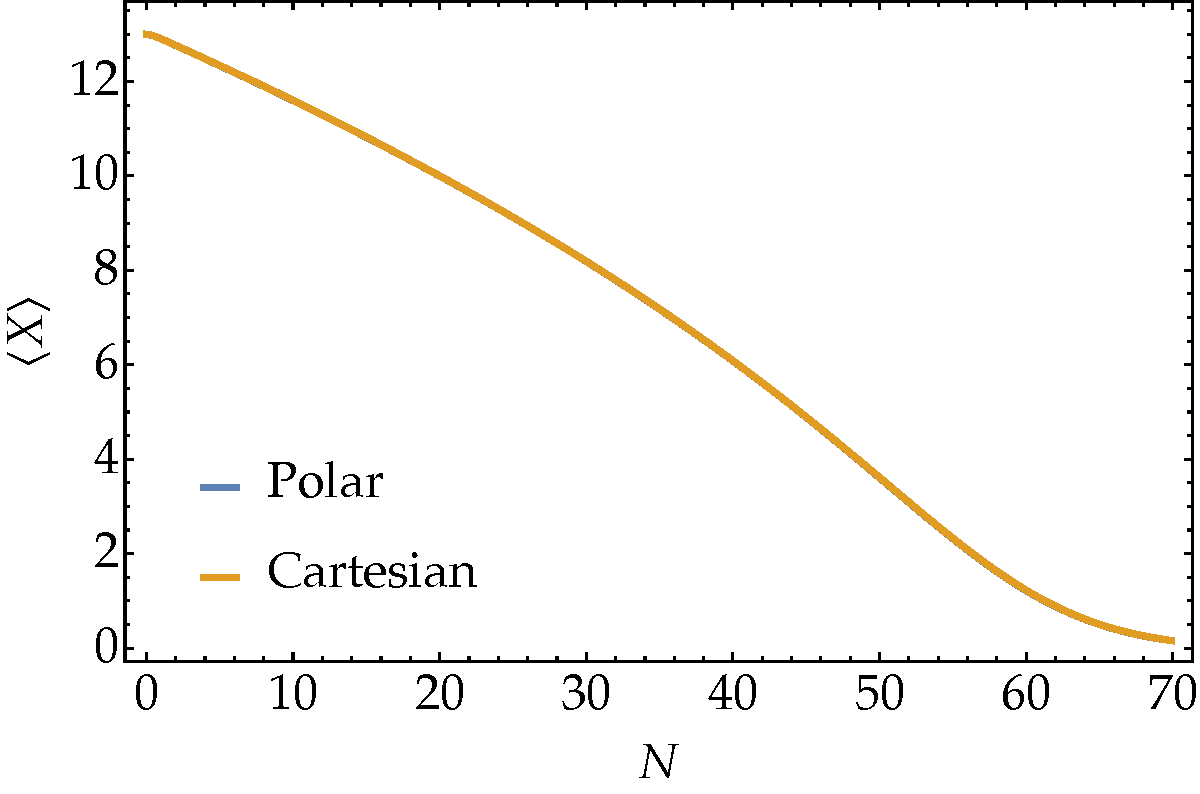
\includegraphics[width=\hsize]{figs/meanX.pdf}
		\end{minipage}
		\begin{minipage}{0.5\hsize}
			\centering
			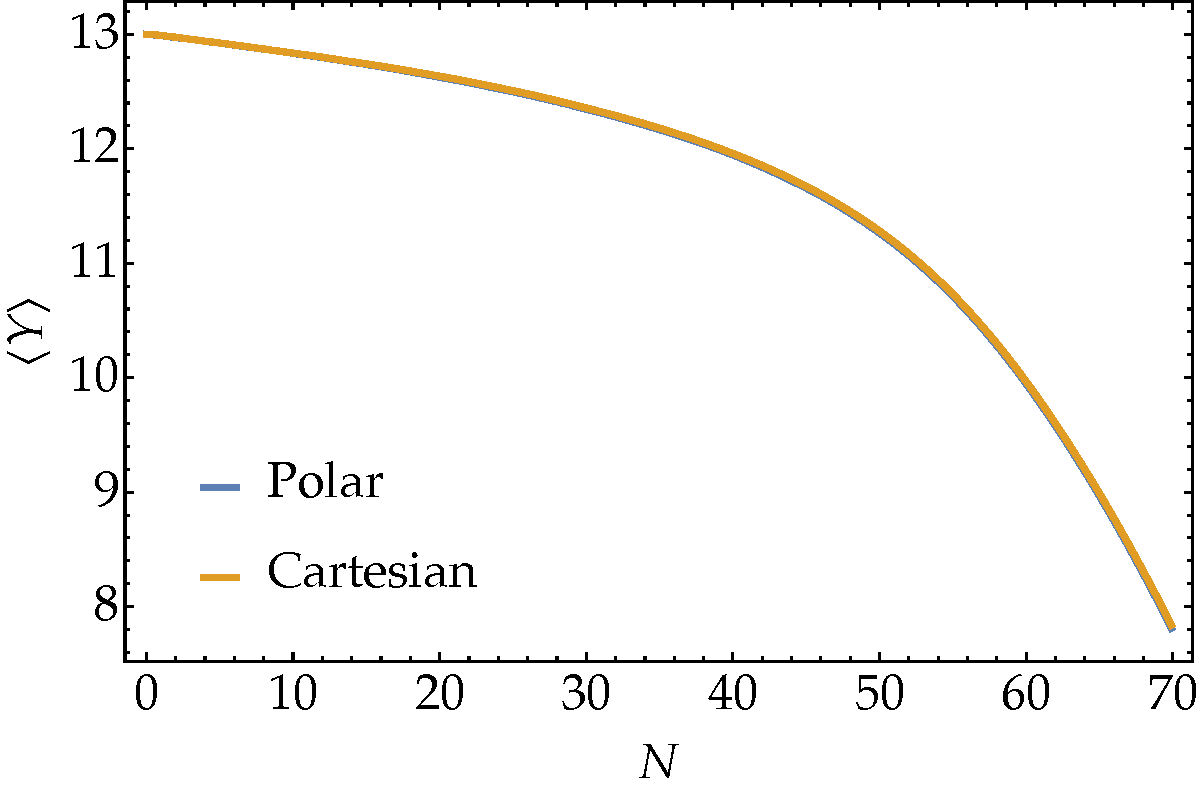
\includegraphics[width=\hsize]{figs/meanY.pdf}
		\end{minipage} \\
		\begin{minipage}{0.5\hsize}
			\centering
			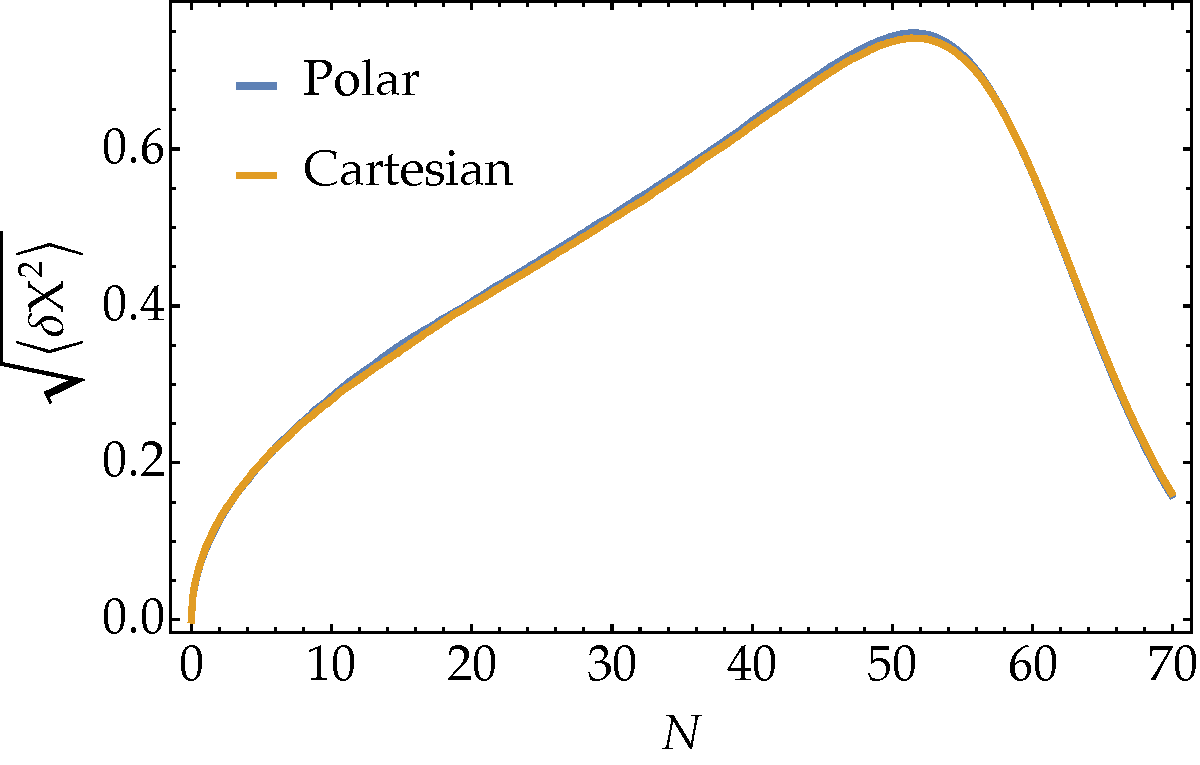
\includegraphics[width=\hsize]{figs/stdX.pdf}
		\end{minipage}
		\begin{minipage}{0.5\hsize}
			\centering
			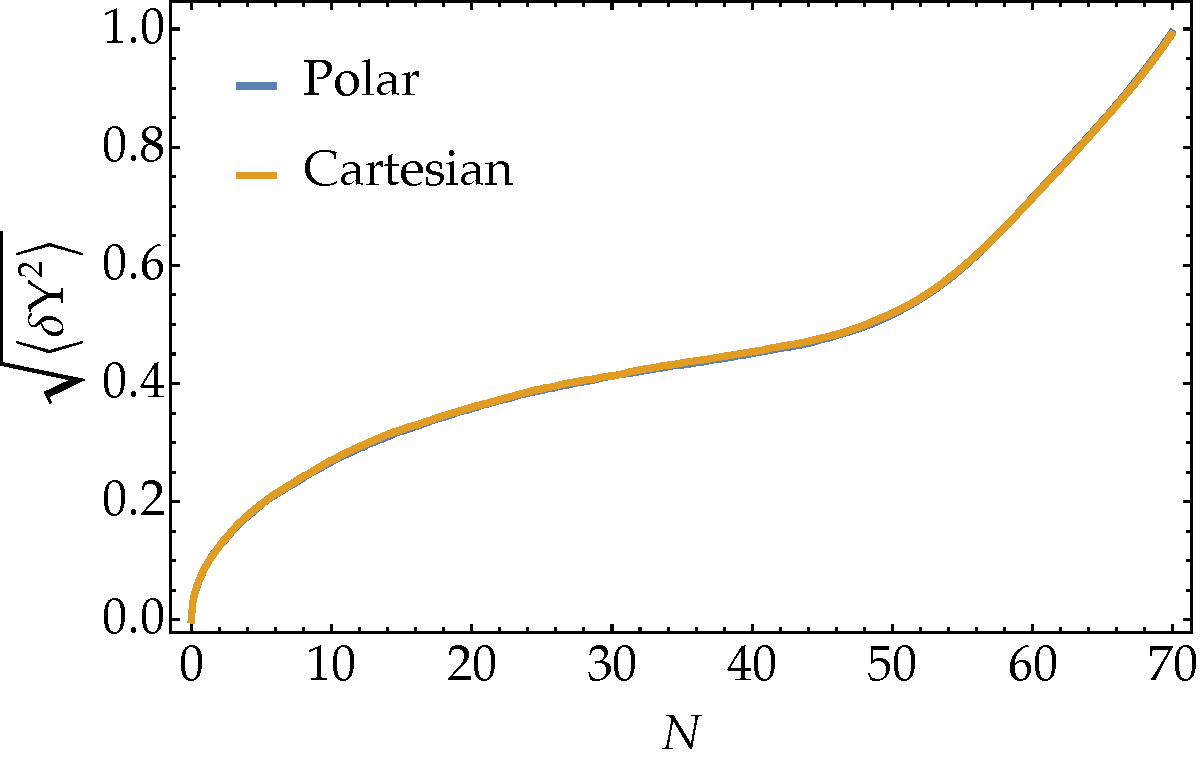
\includegraphics[width=\hsize]{figs/stdY.pdf}
		\end{minipage}
	\end{tabular}
	\caption{The comparison between the polar and Cartesian coordinates. To see the noise effect clearly, we adopt 
	an unrealistically high energy scale as $M=3m=0.1\Mpl$. The initial condition is given by $(X_\text{i},Y_\text{i},\dd X_\text{i}/\dd N,\dd Y_\text{i}/\dd N)
	=(13\Mpl,13\Mpl,0,0)$. The averages are given by 10000 realizations.}
	\label{fig: CvsP}
\end{figure}
		
			


\bigskip
Instead of the differential coefficient, the trivial parallel transported vielbein
\bae{\label{eq: trivial vielbein}
	e^r_1=1, \quad\quad e^\theta_2=1/r, \quad\quad \text{(otherwise)}=0,
}
gives an apparently different Langevin equation. Therefore it can be used to check the numerical code by comparing
with the calculation in the Cartesian coordinate.
For simplicity, we only consider the mass terms for the potential:
\bae{
	V(X,Y)=\frac{1}{2}M^2X^2+\frac{1}{2}m^2Y^2,
}
and we take the massless approximation for the noise term. That is, according to Eq.~(\ref{eq: massless}), 
the Langevin equation reads
\bae{
	\bce{
		\displaystyle
		\dif{\varphi^I}{N}=\frac{\pi^I}{H}+\frac{H}{2\pi}e^I_\alpha\xi_\alpha, \\[10pt]
		\displaystyle
		\dif{\pi^I}{N}=-\gamma^I_{JK}\pi^K\dif{\varphi^J}{N}-3\pi^I-\gamma^{IJ}\frac{V_J}{H}
		=-\gamma^I_{JK}\frac{\pi^J\pi^K}{H}-3\pi^I-\gamma^{IJ}\frac{V_J}{H}-\gamma^I_{JK}\pi^K\frac{H}{2\pi}e^J_\alpha\xi_\alpha, \\[10pt]
		\displaystyle
		\braket{\xi_\alpha(N,\mathbf{x})\xi_\beta(N^\prime,\mathbf{x}^\prime)}=\delta(N-N^\prime)
		\frac{\sin(\sigma aH|\mathbf{x}-\mathbf{x}^\prime|)}{\sigma aH|\mathbf{x}-\mathbf{x}^\prime|},
	}
}
with use of the e-folding number as a time variable. Concretely, considering the one-spatial-point dynamics,
these equations can be written as
\bae{
	\bce{
		\displaystyle
		\dif{r}{N}=\frac{\pi_r}{H}+\frac{H}{2\pi}\xi_1, & 
		\displaystyle
		\dif{\theta}{N}=\frac{\pi_\theta}{H}+\frac{H}{2\pi r}\xi_2, \\[10pt]
		\displaystyle
		\dif{\pi_r}{N}=r\frac{\pi_\theta^2}{H}-3\pi_r-\frac{V_r}{H}+\frac{H}{2\pi}\pi_\theta\xi_2, &
		\displaystyle
		\dif{\pi_\theta}{N}=-\frac{2\pi_r\pi_\theta}{Hr}-3\pi_\theta-\frac{V_\theta}{Hr^2}-\frac{H}{2\pi r}\pi_\theta\xi_1-\frac{H}{2\pi r^2}\pi_r\xi_2, \\[10pt]
		\displaystyle
		\braket{\xi_1(N)\xi_1(N^\prime)}=\braket{\xi_2(N)\xi_2(N^\prime)}=\delta(N-N^\prime), &
		\displaystyle
		\braket{\xi_1(N)\xi_2(N^\prime)}=0,
	}
}
in the polar coordinate, and as
\bae{
	\bce{
		\displaystyle
		\dif{X}{N}=\frac{\pi_X}{H}+\frac{H}{2\pi}\xi_X, &
		\displaystyle
		\dif{Y}{N}=\frac{\pi_Y}{H}+\frac{H}{2\pi}\xi_Y, \\[10pt]
		\displaystyle
		\dif{\pi_X}{N}=-3\pi_X-\frac{V_X}{H}, &
		\displaystyle
		\dif{\pi_Y}{N}=-3\pi_Y-\frac{V_Y}{H}, \\[10pt]
		\displaystyle
		\braket{\xi_X(N)\xi_X(N^\prime)}=\braket{\xi_Y(N)\xi_Y(N^\prime)}=\delta(N-N^\prime), &
		\displaystyle
		\braket{\xi_X(N)\xi_Y(N^\prime)}=0,
	}
}
in the Cartesian coordinate.
Note that, with use of the vielbein~(\ref{eq: trivial vielbein}), the noise $\xi_1$ and $\xi_2$ in the polar coordinate and
$\xi_X$ and $\xi_Y$ in the Cartesian coordinate are not in the same basis, and therefore the above two sets of Langevin equations are
not equivalent any longer. However the difference between them should be slow-roll suppressed because they are caused by 
the slow-roll approximation.
In Fig.~\ref{fig: CvsP}, we show the numerical results in the polar and Cartesian coordinates, and they are well consistent. 



\subsection{EoM vs. effective action}

As a heuristic approach to the stochastic formalism, one can directly divide the scalar EoM into the IR and UV modes
to obtain the Langevin equation. According to Lucas's report, the following Langevin equation can be obtained from this approach.
\bae{\label{eq: heuristic}
	\bce{
		\displaystyle
		\dot{\varphi}^I=\frac{\gamma^{IJ}}{a^3}\varpi_J+\xi^I_Q, \\[10pt]
		\displaystyle
		\dot{\varpi}_I=-a^3V_I-\frac{\gamma^{JK}{}_{,I}}{2a^3}\varpi_J\varpi_K+\xi^P_I,
	}
}
where
\bae{
	\xi^I_Q=-\int\dk\ee^{i\mathbf{k}\cdot\mathbf{x}}\dot{W}_tQ^I_\mathbf{k}, \quad\quad
	\xi^P_I=-\int\dk\ee^{i\mathbf{k}\cdot\mathbf{x}}\dot{W}_tP_I^\mathbf{k}.
}
$Q^I=e^I_\alpha\tilde{Q}_\alpha$ is the UV part of $\phi^I$ following the linearized EoM
\bae{
	D_tD_tQ^I_\mathbf{k}+3HD_tQ^I_\mathbf{k}+\frac{k^2}{a^2}Q^I_\mathbf{k}
	+\left[V^I{}_{;J}-\gamma^I{}_{KLJ}\dot{\varphi}^K\dot{\varphi}^L
	-\frac{1}{a^3}D_t\left(\frac{a^3}{H}\gamma_{JK}\dot{\varphi}^I\dot{\varphi}^K\right)\right]Q^J_\mathbf{k}=0.
}
$P_I$ is the UV part of the conjugate momentum given by
\bae{\label{eq: def of P}
	P_I=-a^3\gamma_{IJ}\dot{\varphi}^JN^{(1)}+a^3\gamma_{IJ,K}\dot{\varphi}^JQ^K+a^3\gamma_{IJ}\dot{Q}^J.
}
In this approach, the noise term is treated as half-quantum and half-classical. That is, the ``clasicall" statistics of the noise $\xi_Q$ and $\xi^P$
is assumed to be given by the ``quantum" correlation of $Q$ or $P$, like as
\bae{
	\braket{\xi^I_Q(t,\mathbf{x})\xi^P_J(t^\prime,\mathbf{x}^\prime)}:=\int\dk\frac{\dd k^\prime}{(2\pi)^3}\ee^{i(\mathbf{k}\cdot{\mathbf{x}}
	+\mathbf{k}^\prime\cdot\mathbf{x}^\prime)}\dot{W}_t\dot{W}_{t^\prime}\braket{Q^I_\mathbf{k}P_J^{\mathbf{k}^\prime}},
}
and so on.

One can see that the form of the Langevin equation~(\ref{eq: heuristic}) is reduced to our result~(\ref{eq: general Langevin})
by relating the quantities as
\bae{\label{eq: redefinition of pi and xi}
	\varpi_I=a^3\gamma_{IJ}\pi^J, \quad\quad \xi^I_Q=e^I_\alpha R_{\alpha A}\xi_A, \quad\quad 
	\xi^P_I=\gamma^K_{IJ}\xi^J_Q\varpi_K+a^3e_{I\alpha}R_{N+\alpha,A}\xi_A.
}
However there is a discrepancy in the noise statistic, particularly related to $\xi^P$.
By definition~(\ref{eq: def of P}), the noise correlation $\braket{\xi_Q\xi^P}$ has three contributions as
\bae{
	\braket{\xi_Q^I\xi^P_J}\propto-a^3\gamma_{JK}\dot{\varphi}^K\braket{Q^IN^{(1)}}+a^3\gamma_{JK,L}\dot{\varphi}^K\braket{Q^IQ^L}
	+a^3\gamma_{JK}\braket{Q^I\dot{Q}^K}.
}
The latter two terms can be reproduced by the redefinition~(\ref{eq: redefinition of pi and xi}),\footnote{Indeed it means that, if one neglects
$N^{(1)}$ term in the definition of $P$ as
\bae{
	P_I\simeq a^3\gamma_{IJ,K}\dot{\varphi}^JQ^K+a^3\gamma_{IJ}\dot{Q}^J, \quad \text{(around the horizon cross $k\sim\sigma aH$),}
}
the noise entering for the scalar fields as $\varphi\to\varphi+Q_{k=\sigma aH}$ consistently reproduces the noise entering for the conjugate momentum
$\varpi\to\varpi+P_{k=\sigma aH}$.
}
but the first term $\propto\braket{Q^IN^{(1)}}=\frac{1}{2\Mpl^2H}\dot{\varphi}_J\braket{Q^IQ^J}$ cannot.
In fact we take the gauge as $N_\text{IR}=1$ and therefore $N^{(1)}$ should be zero on the superhorizon scale.
That may cause this discrepancy.


\newpage
\part{Hamiltonian formalism}

\section{Canonical single field}

Let us start by the canonical single field action
\bae{
	S=\int\dd^4x\sqrt{-g}\left[\frac{\Mpl^2}{2}R-\frac{1}{2}g^{\mu\nu}\partial_\mu\phi\partial_\nu\phi-V(\phi)\right],
}
to see the basic idea of the Hamiltonian approach.
Taking the flat gauge in the ADM form as
\bae{
	\dd s^2=-N^2\dd t^2+a^2\delta_{ij}(\dd x^i+\beta^i\dd t)(\dd x^j+\beta^j\dd t),
}
the conjugate momentum is given by
\bae{
	\pi=\var{S}{\dot{\phi}}=\frac{a^3}{N}(\dot{\phi}-\beta^i\partial_i\phi).
}
Then the Hamiltonian is related with the Lagrangian as
\bae{
	S=\int\dd^4x(\pi\dot{\phi}-\mathcal{H}),
}
where
\bae{
	\mathcal{H}=a^3N\left(\frac{\pi^2}{2a^6}+\frac{1}{2a^2}\partial_i\phi\partial_i\phi+V-\frac{\Mpl^2}{2}R\right)+\pi\beta^i\partial_i\phi.
}
Decomposing physical variables into IR and UV parts as
\bae{
	\phi\to\varphi+Q, \quad \pi\to\varpi+P, \quad N\to N_\text{IR}+\alpha, \quad \beta^i\to a^{-2}\partial_i\psi,
}
the action can be written, up to quadratic orders in $Q$, $P$, $\alpha$, and $\psi$, as
\bae{
	S\simeq& S^{(0)}+S^{(1)}+S^{(2)}, \nonumber \\
	S^{(0)}=&\int\dd^4x\left[\varpi\dot{\varphi}-a^3N_\IR\left(\frac{\varpi^2}{2a^6}+V+\frac{3\Mpl^2H^2}{N_\text{IR}}\right)\right], 
	\label{eq: S0: Hamiltonian} \\
	S^{(1)}=&\int\dd^4x\left[P\left(\dot{\varphi}-\frac{N_\IR}{a^3}\varpi\right)-Q\left(\dot{\varpi}+a^3N_\IR V^\prime\right)
	-a^3\alpha\left(\frac{\varpi^2}{2a^6}+V-\frac{3\Mpl^2H^2}{N_\IR}\right)\right], 
	\label{eq: S1: Hamiltonian} \\
	S^{(2)}=&\int\dd^4x\left[-\frac{3\Mpl^2H^2a^3}{N_\IR^3}\alpha^2-a^3\alpha\left(\frac{\varpi P}{a^6}+V^\prime Q
	+\frac{2\Mpl^2H}{N_\IR^2}\frac{\nabla^2}{a^2}\psi\right)+\varpi Q\frac{\nabla^2}{a^2}\psi\right. \nonumber \\
	&\left.-a^3N_\IR\left(\frac{P^2}{2a^6}-\frac{1}{2a^2}Q\nabla^2Q+\frac{1}{2}V^{\prime\prime}Q^2\right)+P\dot{Q}\right],
	\label{eq: S2: Hamiltonian}
}
where gradients of IR modes are neglected. Also the Hubble parameter is here defined by $H=\dot{a}/a$ for any lapse $N_\IR$ 
(e.g. $H=1$ for the e-folding time).
Note that the variation of $S^{(1)}$ w.r.t. the perturbations $P$, $Q$, and $\alpha$ gives the classical EoM and energy constraint:
\bae{\label{eq: classical EoM}
	\bce{
		\dps
		\var{S^{(1)}}{P}=\dot{\varphi}-\frac{N_\IR}{a^3}\varpi\approx0, \\[10pt]
		\dps
		\var{S^{(1)}}{Q}=-\dot{\varpi}-a^3N_\IR V^\prime\approx0, \\[10pt]
		\dps
		\var{S^{(1)}}{\alpha}=-a^3\left(\frac{\varpi^2}{2a^6}+V-\frac{3\Mpl^2H^2}{N_\IR}\right)\approx0.
	}
}
Here we used $\approx$ for equalities which hold up to noise. Actually it will be verified that the Friedmann equation 
\bae{\label{eq: Friedmann}
	F:=\frac{\varpi^2}{2a^6}+V-\frac{3\Mpl^2H^2}{N_\IR}=0
}
does hold even under the existence of the noise terms.

In the action~(\ref{eq: S0: Hamiltonian})--(\ref{eq: S2: Hamiltonian}), $\alpha$ and $\psi$ appear as Lagrange multipliers, that is,
the corresponding terms do not include any time derivative. Therefore they can be integrated out in advance, which is equivalent to
substituting the solutions of the corresponding constraints (actually we only need the second constraint)
\bae{
	\bce{
		\dps
		\var{S}{\alpha}=-\frac{6\Mpl^2H^2a^3}{N_\IR^3}\alpha-a^3\left(F+\frac{\varpi P}{a^6}+V^\prime Q
		+\frac{2\Mpl^2H}{N_\IR^2}\frac{\nabla^2}{a^2}\psi\right)=0, \\[10pt]
		\dps
		\var{S}{\psi}=-\frac{2\Mpl^2Ha^3}{N_\IR^2}\frac{\nabla^2}{a^2}\alpha+\varpi\frac{\nabla^2}{a^2}Q=0,
		\quad \Rightarrow \quad \alpha=\frac{N_\IR^2}{2\Mpl^2Ha^3}\varpi Q.
	}
}
After that, the remained action reads
\bae{
	S^{(0)}=&\int\dd^4x\left[\varpi\dot{\varphi}-a^3N_\IR\left(\frac{\varpi^2}{2a^6}+V+\frac{3\Mpl^2H^2}{N_\IR^2}\right)\right], \\
	S^{(1)}=&\int\dd^4xQ_XE_X, \quad\quad S^{(2)}=\int\dd^4x\frac{1}{2}Q_X\Lambda_{XY}Q_Y,
}
where indices $X$ and $Y$ represent $Q$ or $P$ with
\bae{
	\bce{
		\dps
		Q_Q=Q, \quad\quad Q_P=P, \\[10pt]
		\dps
		E_Q=-\left(\dot{\varpi}+a^3N_\IR V^\prime+\frac{N_\IR^2}{2\Mpl^2H}\varpi F\right), \quad\quad
		E_P=\dot{\varphi}-\frac{N_\IR}{a^3}\varpi, \\[10pt]
		\dps
		\Lambda=
		\bpme{
			-\frac{N_\IR}{a^3} & -M_{PQ}^2+\partial_t \\
			-M_{PQ}^2-\partial_t & a^3N_\IR\left(\frac{\nabla^2}{a^2}-M_{QQ}^2\right)
		}, \\[10pt]
		\dps
		M_{PQ}^2=\frac{N_\IR^2}{2\Mpl^2Ha^6}\varpi^2, \quad\quad 
		M_{QQ}^2=V^{\prime\prime}+\frac{N_\IR}{\Mpl^2Ha^3}\varpi V^\prime+\frac{3}{2\Mpl^2a^6}\varpi^2.
	}
}

We will later check that the UV modes follow the EoM
\bae{\label{eq: QP EoM}
	\Lambda_{XY}Q_Y=0, \quad \Leftrightarrow \quad
	\bce{
		\dps
		\dot{Q}=\frac{N_\IR}{a^3}P+M_{PQ}^2Q, \\[10pt]
		\dps
		\dot{P}=-M_{PQ}^2P+a^2N_\IR\left(\frac{\nabla^2}{a^2}-M_{QQ}^2\right)Q.
	}
}
It can be verified that it is equivalent to the well-known EoM
\bae{\label{eq: standard Q EoM}
	\frac{1}{N_\IR^2}\ddot{Q}+\frac{1}{N_\IR^2}\left(3H-\frac{\dot{N}_\IR}{N_\IR}\right)\dot{Q}-\frac{\nabla^2}{a^2}Q
	+\left[V^{\prime\prime}-\frac{1}{a^3N_\IR\Mpl^2}\partial_t\left(\frac{N_\IR}{a^3H}\varpi^2\right)\right]Q=0,
}
up to noise.
First, from Eq.~(\ref{eq: QP EoM}), one obtains
\bae{\label{eq: Q EoM before using classical EoM}
	\frac{1}{N_\IR^2}\ddot{Q}+\frac{1}{N_\IR^2}\left(3H-\frac{\dot{N}_\IR}{N_\IR}\right)\dot{Q}-\frac{\nabla^2}{a^2}Q
	-\frac{1}{a^3N_\IR}\left[\partial_t\left(\frac{a^3}{N_\IR}M_{PQ}^2\right)+\frac{a^3}{N_\IR}M_{PQ}^4-a^3N_\IR M_{QQ}^2\right]Q=0.
}
On the other hand, the time derivative of the Friedmann equation~(\ref{eq: Friedmann}) gives
\bae{
	\frac{6\Mpl^2H^2}{N_\IR^2}\left(\frac{\dot{H}}{H}-\frac{\dot{N}_\IR}{N_\IR}\right)
	=\frac{\varpi\dot{\varpi}}{a^6}-3H\frac{\varpi^2}{a^6}+V^\prime\dot{\varphi}.
}
With use of the classical EoM~(\ref{eq: classical EoM}), it reads
\bae{
	\frac{\dot{H}}{H}-\frac{\dot{N}_\IR}{N_\IR}=\frac{N_\IR^2}{2\Mpl^2Ha^6}\varpi^2.
}
Then $M_{PQ}^4$ can be rewritten as
\bae{
	M_{PQ}^4=M_{PQ}^2\left(\frac{\dot{H}}{H}-\frac{\dot{N}_\IR}{N_\IR}\right).
}
Finally, using the classical EoM for $V^\prime$ in $M_{QQ}^2$, one can find that 
the last part of Eq.~(\ref{eq: Q EoM before using classical EoM}) reads
\bae{
	-\frac{1}{a^3N_\IR}\left[\partial_t\left(\frac{a^3}{N_\IR}M_{PQ}^2\right)+\frac{a^3}{N_\IR}M_{PQ}^4-a^3N_\IR M_{QQ}^2\right]Q
	=\left[V^{\prime\prime}-\frac{a^3}{N_\IR}\partial_t\left(\frac{2a^3}{N_\IR}M_{PQ}^2\right)\right]Q,
}
reproducing the standard one~(\ref{eq: standard Q EoM}). To obtain this result, we used the classical EoM~(\ref{eq: classical EoM}) which
holds only if we neglect the noise terms. It can be justified as follows. The noise itself comes from the UV modes $Q$ or $P$, while
we here consider the action up to the quadratic order in them. Therefore the EoM for $Q$ and $P$ should be linear in them,
and the noise contribution for the coefficients of the EoM can be consistently neglected.





\subsection{Effective action}

To obtain the effective action for IR modes, we consider the path integral along with a closed time path similarly to the Lagrangian formalism:
\bae{
	Z[\calJ^\pm_{Q,P},\scrJ^\pm_{Q,P}]=&\calN\int\scrD\varphi^\pm\scrD\varpi^\pm\ee^{i\left(S^{(0),+}-S^{(0),-}+\calJ_{Xa}\varphi_X{}^a\right)} 
	\nonumber \\
	&\times\int\scrD Q^\pm\scrD P^\pm\exp\left[i\left(Q_{Xa}E_X{}^a+\frac{1}{2}Q_{Xa}\Lambda_{XY}{}^a{}_bQ_Y{}^b+\scrJ_{Xa}Q_X{}^a\right)\right].
}
$Q$ and $P$ can be integrated out as
\bae{
	Z[\calJ_{Q,P}^\pm,\scrJ_{Q,P}^\pm]=&\calN\int\scrD\varphi^\pm\scrD\varpi^\pm\ee^{i\left(S^{(0),+}-S^{(0),-}+\calJ_{Xa}\varphi_X{}^a\right)} 
	\nonumber \\
	&\times\exp\left[-\frac{i}{2}(E_{Xa}+\scrJ_{Xa})(\Lambda^{-1})_{XY}{}^a{}_b(E_Y{}^b+\scrJ_Y{}^b)\right].
}
Then let us adopt the classicalization assumption for IR modes, that is, the integration w.r.t. $\varphi$ and $\varpi$ leads
the replacement of them to the vev $\braket{\varphi}_\calJ$ and $\braket{\varpi}_\calJ$ under the existence of the source term $\calJ$.
Therefore the partition function can be approximated as
\bae{\label{eq: Z in Hamiltonian}
	Z[\calJ^\pm_{Q,P},\scrJ^\pm_{Q,P}]\simeq&\calN\exp\left[i\left(S^{(0)}[\braket{\varphi^+}_\calJ,\braket{\varpi^+}_\calJ]
	-S^{(0)}[\braket{\varphi^-}_\calJ,\braket{\varpi^-}_\calJ]+\calJ_{Xa}\braket{\varphi_X{}^a}_\calJ \right.\right.\nonumber \\
	&\left.\left.-\frac{1}{2}(E_{Xa}+\scrJ_{Xa})(\Lambda^{-1})_{XY}{}^a{}_b(E_X{}^b+\scrJ_X{}^b)\right)\right].
}
Defining $iW$ by its exponent as
\bae{
	W[\calJ^\pm_{Q,P},\scrJ^\pm_{Q,P}]=&S^{(0)}[\braket{\varphi^+}_\calJ,\braket{\varpi^+}_\calJ]
	-S^{(0)}[\braket{\varphi^-}_\calJ,\braket{\varpi^-}_\calJ]+\calJ_{Xa}\braket{\varphi_X{}^a}_\calJ \nonumber \\
	&-\frac{1}{2}(E_{Xa}+\scrJ_{Xa})(\Lambda^{-1})_{XY}{}^a{}_b(E_X{}^b+\scrJ_X{}^b),
}
the effective action $\Gamma$ is given by its Legendre transformation
\bae{
	\Gamma[\braket{\varphi^\pm},\braket{\varpi^\pm},\braket{Q^\pm},\braket{P^\pm}]=W[\calJ^\pm_{Q,P},\scrJ^\pm_{Q,P}]
	-\calJ_{Xa}\braket{\varphi_X{}^a}-\scrJ_{Xa}\braket{Q_X{}^a}.
}
Here the field vev and the source term are related by
\bae{
	\braket{\varphi_X{}^a}=\var{W}{\calJ_{Xa}}, \quad\quad \braket{Q_X{}^a}=\var{W}{\scrJ_{Xa}}
	=-(\Lambda^{-1})_{XY}{}^a{}_b(E_Y{}^b+\scrJ_Y{}^b).
}
Therefore the explicit form of the effective action is
\bae{
	\Gamma[\braket{\varphi^\pm},\braket{\varpi^\pm},\braket{Q^\pm},\braket{P^\pm}]=&S^{(0)}[\braket{\varphi^+},\braket{\varpi^+}]
	-S^{(0)}[\braket{\varphi^-},\braket{\varpi^-}] \nonumber \\
	&+\frac{1}{2}\braket{Q_{Xa}}\Lambda_{XY}{}^a{}_b\braket{Q_Y{}^b}+E_{Xa}\braket{Q_X{}^a}.
}
The vev of $Q$ and $P$ is solved as a stationary point of the effective action:
\bae{
	\braket{Q_X{}^a}=-(\Lambda^{-1})_{XY}{}^a{}_bE_Y{}^b.
}
Substituting it back into the effective action, one finally obtains the effective action for IR modes as
\bae{
	\Gamma_\IR[\braket{\varphi^\pm},\braket{\varpi^\pm}]=S^{(0)}[\braket{\varphi^+},\braket{\varpi^+}]
	-S^{(0)}[\braket{\varphi^-},\braket{\varpi^-}]-\frac{1}{2}E_{Xa}(\Lambda^{-1})_{XY}{}^a{}_bE_Y{}^b.
}
Particularly the last term $\SIA=-\frac{1}{2}E_{Xa}(\Lambda^{-1})_{XY}{}^a{}_bE_Y{}^b$ is called \emph{influence action}, which
exhibits the effect of the horizon-exiting UV modes. We will omit brackets hereafter for conciseness.




\subsection{Influence action}

In the influence action, $\Lambda^{-1}$ has not been clarified yet.
By taking the variation of the partition function~(\ref{eq: Z in Hamiltonian}), one finds that $\Lambda^{-1}$ is nothing but the time-ordered two
point function of $Q$ or $P$:
\bae{
	\braket{T_CQ_X{}^a(x)Q_{Yb}(x^\prime)}=\left.\frac{1}{i}\var{}{\scrJ_{Xa}(x)}\frac{1}{i}\var{}{\scrJ_Y{}^b(x^\prime)}Z\right|_{\calJ=\scrJ=0}
	=i(\Lambda^{-1})_{XY}{}^a{}_b(x,x^\prime).
}
Here the time-ordering should be defined along with the closed time path $C$ as
\bae{
	T_CQ_X{}^a(x)Q_{Yb}(x^\prime)=
	\bce{
		\dps
		\theta(t-t^\prime)Q_X{}^a(x)Q_{Yb}(x^\prime)+\theta(t^\prime-t)Q_{Yb}(x^\prime)Q_X{}^a(x), & 
		\dps
		(a=+,b=+), \\
		\dps
		Q_{Yb}(x^\prime)Q_X{}^a(x), & 
		\dps
		(a=+,b=-), \\
		\dps
		Q_X{}^a(x)Q_{Yb}(x^\prime), &
		\dps
		(a=-,b=+), \\
		\dps
		\theta(t^\prime-t)Q_X{}^a(x)Q_{Yb}(x^\prime)+\theta(t-t^\prime)Q_{Yb}(x^\prime)Q_X{}^a(x), & 
		\dps
		(a=-,b=-).
	}
}
Expanding the field operator $\hat{Q}_X(x)$ as 
\bae{
	\hat{Q}_X(x)=\int\dk W_t\left[\phi_X(t,k)\hat{a}(\mathbf{k})\ee^{i\mathbf{k}\cdot\mathbf{x}}
	+\phi_X^*(t,k)\hat{a}^\dagger(\mathbf{k})\ee^{-i\mathbf{k}\cdot\mathbf{x}}\right],
}
the propagator reads
\bae{
	&\braket{T_CQ_X{}^a(x)Q_{Yb}(x^\prime)}=\int\dk W_tW_{t^\prime} \nonumber \\
	&\times\bce{
		\dps
		\theta(t-t^\prime)\phi_X{}^a(t,k)\phi^*_{Yb}(t^\prime,k)+\theta(t^\prime-t)\phi_{Yb}(t^\prime,k)\phi^*_X{}^a(t,k), & 
		\dps
		(a=+,b=+), \\
		\dps
		\phi_{Yb}(t^\prime,k)\phi_X{}^a(t,k), & 
		\dps
		(a=+,b=-), \\
		\dps
		\phi_X{}^a(t,k)\phi^*_{Yb}(t^\prime,k), &
		\dps
		(a=-,b=+), \\
		\dps
		\theta(t^\prime-t)\phi_X{}^a(t,k)\phi^*_{Yb}(t^\prime,k)+\theta(t-t^\prime)\phi_{Yb}(t^\prime,k)\phi^*_X{}^a(t,k), & 
		\dps
		(a=-,b=-).
	}
}
The mode function $\phi_X(t,k)$ should satisfy the subhorizon EoM
\bae{
	\Lambda_{XY}\phi_Y(t,k)=0. \quad \Leftrightarrow \quad
	\bce{
		\dps
		\dot{\phi}(t,k)=\frac{N_\IR}{a^3}\pi(t,k)+M_{PQ}^2\phi(t,k), \\[10pt]
		\dps
		\dot{\pi}(t,k)=-M_{PQ}^2\pi(t,k)-aN_\IR^2k^2\phi(t,k)-M_{QQ}^2\phi(t,k).
	}
}

Now one obtains the explicit expression of the influence action as
\bae{
	\SIA=&-\frac{1}{2}E_{Xa}(\Lambda^{-1})_{XY}{}^a{}_bE_Y{}^b \nonumber \\
	=&\frac{i}{2}\int\dd^4x\dd^4x^\prime\int\dk E_{Xa}(x)W_t \nonumber \\
	&\times\bpme{
		\begin{array}{c}
			\theta(t-t^\prime)\phi_X(t,k)\phi^*_Y(t^\prime,k)\ee^{i\mathbf{k}\cdot(\mathbf{x}-\mathbf{x}^\prime)} \\
			+\theta(t^\prime-t)\phi_Y(t^\prime,k)\phi^*_X(t,k)\ee^{i\mathbf{k}\cdot(\mathbf{x}^\prime-\mathbf{x})}
		\end{array} &
		-\phi_Y(t^\prime,k)\phi^*_X(t,k)\ee^{i\mathbf{k}\cdot(\mathbf{x}^\prime-\mathbf{x})} \\
		\phi_X(t,k)\phi^*_Y(t^\prime,k)\ee^{i\mathbf{k}\cdot(\mathbf{x}-\mathbf{x}^\prime)} &
		\begin{array}{c}
			-\theta(t^\prime-t)\phi_X(t,k)\phi^*_Y(t^\prime,k)\ee^{i\mathbf{k}\cdot(\mathbf{x}-\mathbf{x}^\prime)} \\
			-\theta(t-t^\prime)\phi_Y(t^\prime,k)\phi^*_X(t,k)\ee^{i\mathbf{k}\cdot(\mathbf{x}^\prime-\mathbf{x})}
		\end{array}
	}{}^a{}_b \nonumber \\
	&\times W_{t^\prime}E_Y{}^b(x^\prime).
}
From the orthogonality between IR and UV modes, we will drop terms without any time derivative. Note that each $E_X$ includes only one
time-derivative term as
\bae{
	E_Q\supset-\dot{\varpi}, \quad\quad E_P\supset\dot{\varphi},
}
and let us rewrite it as
\bae{
	E_X\supset\dot{\varphi}_{\bar{X}}
}
with a barred index defined by
\bae{
	\varphi_{\bar{Q}}=-\varpi, \quad\quad \varphi_{\bar{P}}=\varphi.
}
Then the non-vanishing terms in the influence action come from
\bae{
	\SIA=&\frac{i}{2}\int\dd^4x\dd^4x^\prime\int\dk\dot{\varphi}_{\bar{X}a}(x)W_t \nonumber \\
	&\times\bpme{
		\begin{array}{c}
			\theta(t-t^\prime)\phi_X(t,k)\phi^*_Y(t^\prime,k)\ee^{i\mathbf{k}\cdot(\mathbf{x}-\mathbf{x}^\prime)} \\
			+\theta(t^\prime-t)\phi_Y(t^\prime,k)\phi^*_X(t,k)\ee^{i\mathbf{k}\cdot(\mathbf{x}^\prime-\mathbf{x})}
		\end{array} &
		-\phi_Y(t^\prime,k)\phi^*_X(t,k)\ee^{i\mathbf{k}\cdot(\mathbf{x}^\prime-\mathbf{x})} \\
		\phi_X(t,k)\phi^*_Y(t^\prime,k)\ee^{i\mathbf{k}\cdot(\mathbf{x}-\mathbf{x}^\prime)} &
		\begin{array}{c}
			-\theta(t^\prime-t)\phi_X(t,k)\phi^*_Y(t^\prime,k)\ee^{i\mathbf{k}\cdot(\mathbf{x}-\mathbf{x}^\prime)} \\
			-\theta(t-t^\prime)\phi_Y(t^\prime,k)\phi^*_X(t,k)\ee^{i\mathbf{k}\cdot(\mathbf{x}^\prime-\mathbf{x})}
		\end{array}
	}{}^a{}_b \nonumber \\
	&\times W_{t^\prime}\dot{\varphi}_{\bar{Y}}{}^b(x^\prime).
}
Integrating by parts and dropping terms with $W$ which is not time-differentiated, it reads
\bae{
	\SIA=&\frac{i}{2}\int\dd^4x\dd^4x^\prime\int\dk\varphi_{\bar{X}a}(x)\dot{W}_t \nonumber \\
	&\times\bpme{
		\begin{array}{c}
			\theta(t-t^\prime)\phi_X(t,k)\phi^*_Y(t^\prime,k)\ee^{i\mathbf{k}\cdot(\mathbf{x}-\mathbf{x}^\prime)} \\
			+\theta(t^\prime-t)\phi_Y(t^\prime,k)\phi^*_X(t,k)\ee^{i\mathbf{k}\cdot(\mathbf{x}^\prime-\mathbf{x})}
		\end{array} &
		-\phi_Y(t^\prime,k)\phi^*_X(t,k)\ee^{i\mathbf{k}\cdot(\mathbf{x}^\prime-\mathbf{x})} \\
		\phi_X(t,k)\phi^*_Y(t^\prime,k)\ee^{i\mathbf{k}\cdot(\mathbf{x}-\mathbf{x}^\prime)} &
		\begin{array}{c}
			-\theta(t^\prime-t)\phi_X(t,k)\phi^*_Y(t^\prime,k)\ee^{i\mathbf{k}\cdot(\mathbf{x}-\mathbf{x}^\prime)} \\
			-\theta(t-t^\prime)\phi_Y(t^\prime,k)\phi^*_X(t,k)\ee^{i\mathbf{k}\cdot(\mathbf{x}^\prime-\mathbf{x})}
		\end{array}
	}{}^a{}_b \nonumber \\
	&\times \dot{W}_{t^\prime}\varphi_{\bar{Y}}{}^b(x^\prime).
}
Finally, moving to the Keldysh basis 
\bae{
	\bpme{
		\varphi^+ \\ \varphi^-
	}
	=\bpme{
		1 & 1/2 \\
		1 & -1/2
	}\bpme{
		\bar{\varphi} \\ \varphi^\Delta
	},
}
the influence action is given by
\bae{
	\SIA=\frac{i}{2}\int\dd^4x\dd^4x^\prime\varphi_{\bar{X}}^\Delta(x)\Re[\Pi_{XY}(x,x^\prime)]\varphi_{\bar{Y}}^\Delta(x^\prime)
	-2\int\dd^4x\dd^4x^\prime\theta(t-t^\prime)\varphi_{\bar{X}}^\Delta(x)\Im[\Pi_{XY}(x,x^\prime)]\bar{\varphi}_{\bar{Y}}(x^\prime),
}
where
\bae{
	\Pi_{XY}(x,x^\prime)=\int\dk\ee^{i\mathbf{k}\cdot(\mathbf{x}-\mathbf{x}^\prime)}\dot{W}_t\dot{W}_{t^\prime}\phi_X(t,k)\phi_Y^*(t^\prime,k).
}




\subsection{Fluctuation}

As previously seen, the noise terms come from the imaginary part of the influence action.
Introducing Gaussian auxiliary fields $\xi_X$, the imaginary action can be rewritten by the real action as
\bae{
	\ee^{i\SIA}\propto\ee^{-\Im[\SIA]}=&\exp\left[-\frac{1}{2}\int\dd^4x\dd^4x^\prime
	\varphi_{\bar{X}}^\Delta\Re[\Pi_{XY}(x,x^\prime)]\varphi_{\bar{Y}}^\Delta\right] \nonumber \\
	=&\calN\int\scrD\xi_Q\scrD\xi_P\exp\left[-\frac{1}{2}\int\dd^4x\dd^4x^\prime\left(\xi_X(x)(\Re\Pi^{-1})_{XY}(x,x^\prime)\xi_Y(x^\prime)\right)
	\right.\nonumber \\
	&\left.+i\int\dd^4x\xi_X(x)\varphi^\Delta_{\bar{X}}(x)\right]
}
The second line represents the Gaussian statistics of the noise as
\bae{
	\braket{\xi_X(x)}=0, \quad\quad \braket{\xi_X(x)\xi_Y(x^\prime)}=\Re[\Pi_{XY}(x,x^\prime)],
}
and the third line shows the coupling between the field and the noise. That is, the real effective action is given by
\bae{
	S_\text{eff}=S^{(0),+}-S^{(0),-}+\int\dd^4x\xi_X(x)\varphi^\Delta_{\bar{X}}(x).
}
Its variation w.r.t. $\varphi^\Delta$, $\varpi^\Delta$, and $N_\IR^\Delta$ at $\varphi_X^+=\varphi_X^-$ gives 
the Langevin equation and the Friedmann constraint
\bae{
	\bce{
		\dps
		\left.\var{S_\text{eff}}{\varpi^\Delta}\right|_{\varphi_X^+=\varphi_X^-}: \quad \dot{\bar{\varphi}}=\frac{N_\IR}{a^3}\bar{\varpi}+\xi_Q, \\[10pt]
		\dps
		\left.\var{S_\text{eff}}{\varphi^\Delta}\right|_{\varphi_X^+=\varphi_X^-}: \quad 
		\dot{\bar{\varpi}}=-a^3N_\IR V^\prime+\xi_P, \\[10pt]
		\dps
		\left.\var{S_\text{eff}}{N_\IR^\Delta}\right|_{\varphi_X^+=\varphi_X^-}: \quad
		\frac{3\Mpl^2H^2}{N_\IR^2}=\frac{\bar{\varpi}^2}{2a^6}+V.
	}
}



\subsection{Dissipation}

According to Morikawa~\cite{Morikawa:1989xz}, the real part of the influence action gives the intrinsic dissipation and mass shift 
caused by the same origin as the fluctuation. Including this, the full Langevin equations obviously read
\bae{
	\bce{
		\dps
		\dot{\varphi}=\frac{N_\IR}{a^3}\varpi+\xi_Q+2\int^t\dd^4x^\prime\Im[\Pi_{QQ}(x,x^\prime)]\varpi(x^\prime)
		-2\int^t\dd^4x^\prime\Im[\Pi_{QP}(x,x^\prime)]\varphi(x^\prime), \\[10pt]
		\dps
		\dot{\varpi}=-a^3N_\IR V^\prime+\xi_P+2\int^t\dd^4x^\prime\Im[\Pi_{PQ}(x,x^\prime)]\varpi(x^\prime)
		-2\int^t\dd^4x^\prime\Im[\Pi_{PP}(x,x^\prime)]\varphi(x^\prime).
	}
}

Let us go further with several assumptions to see the effect of these new terms more intuitively. 
Adopting a step function for the window as $W_t=\theta(k-\sigma aH)$, one obtains
\bae{
	\Pi_{XY}(x,x^\prime)=\frac{\dot{k}_\sigma}{k_\sigma}\frac{\sin(k_\sigma r)}{k_\sigma r}\calP_{XY}(k_\sigma)\delta(t-t^\prime),
}
where
\bae{
	k_\sigma=\sigma aH, \quad\quad r=|\mathbf{x}-\mathbf{x}^\prime|, \quad\quad \calP_{XY}=\frac{k^3}{2\pi^2}Q_X(t,k)Q_Y^*(t,k).
}
Obviously $\calP_{QQ}$ and $\calP_{PP}$ are real so that $\Im[\Pi_{QQ}]=\Im[\Pi_{PP}]=0$.
Also since we are considering coarse-grained fields, $\sin(k_\sigma r)/k_\sigma r$ would be approximated by $\theta(1-k_\sigma r)$.
Therefore, noting that
\bae{\label{eq: edge integral of delta}
	\int^t\dd t^\prime f(t^\prime)\delta(t-t^\prime)=\frac{1}{2}f(t),
}
and 
\bae{\label{eq: tophat approx}
	\varphi(x^\prime)\simeq\varphi(x), \quad\quad \text{(for $|\mathbf{x}-\mathbf{x}^\prime|<k_\sigma^{-1}$)},
}
(\Blue{this approximation seems to be bad...})
the Langevin equations read
\bae{
	\bce{
		\dps
		\dot{\varphi}=\frac{N_\IR}{a^3}\varpi+\xi_Q-\frac{4\pi}{3k_\sigma^3}\frac{\dot{k}_\sigma}{k_\sigma}\Im[\calP_{QP}]\varphi, \\[10pt]
		\dps
		\dot{\varpi}=-a^3N_\IR V^\prime+\xi_P+\frac{4\pi}{3k_\sigma^3}\frac{\dot{k}_\sigma}{k_\sigma}\Im[\calP_{PQ}]\varpi.
	}
}

Hereafter we will use the cosmic time $N_\IR=1$ for simplicity.
In the constant-mass slow-roll limit, the solution for the mode function is given by
\bae{
	\phi(t,k)=\frac{1}{a}\sqrt{\frac{\pi}{4k}}\sqrt{x}H_\nu^{(1)}(x), \quad\quad 
	\left(\text{$x=-k\tau$ and $\nu=\sqrt{\frac{9}{4}-\frac{m^2}{H^2}}$}\right),
}
where $\tau$ is a conformal time with $N_\IR=a$ and $H_\nu^{(1)}$ is the Hankel function of the first kind.
For this solution, the following relation holds at the horizon cross.
\bae{
	\left.\dot{\phi}(t,k)\right|_{k=k_\sigma}=q_\nu\phi(t,k_\sigma),
}
where
\Blue{
\bae{
	q_\nu=-H\left(\frac{3}{2}-\nu+\sigma\frac{H_{\nu-1}^{(1)}(\sigma)}{H_\nu^{(1)}(\sigma)}\right)
	\to -H\left(\sigma^2+i\sigma^3+\mathcal{O}(\sigma^4)\right),
}}
in the massless limit $\nu\to3/2$.
If one neglects $M_{PQ}^2$ which is slow-roll suppressed, $P$ is given by $a^3\dot{Q}$ and therefore
\Blue{
\bae{\label{eq: calPQP}
	\Im[\calP_{QP}(k_\sigma)]=-\Im[\calP_{PQ}(k_\sigma)]=\frac{k_\sigma^3}{H^2}\calP_\phi(k_\sigma)+\mathcal{O}(\sigma^4).
}}
With use of the massless solution $\calP_\phi\to(H/2\pi)^2$ and the relation $\dot{k}_\sigma/k_\sigma=H$ which holds in the slow-roll limit,
the Langevin equations are finally reduced to
\Blue{
\bae{
	\bce{
		\dps
		\dot{\varphi}=\frac{1}{a^3}\varpi+\xi_Q-\frac{H}{3\pi}\varphi, \\[10pt]
		\dps
		\dot{\varpi}=-a^3V^\prime+\xi_P-\frac{H}{3\pi}\varpi,
	}
}}
which can be summarized as,
\Blue{
\bae{
	\ddot{\varphi}+\left(3+\frac{2}{3\pi}\right)H\dot{\varphi}+V^\prime+\frac{9\pi+1}{9\pi^2}H^2\varphi
	=\dot{\xi}_Q+\left(3+\frac{1}{3\pi}\right)H\xi_Q+\frac{1}{a^3}\xi_P.
}}

Except for noise, the real part of the influence action gives rise to the additional dissipation $\frac{2}{3\pi}H\dot{\varphi}$ and
the mass shift $\delta m^2=\frac{9\pi+1}{9\pi^2}H^2$ for background fields. \sout{Note that the sign of the dissipation is opposite to the standard one.
According to Morikawa~\cite{Morikawa:1989xz}, it reflects that the Hubble noise rather injects energy into the system.}
The mass shift $\delta m^2$ does not seem to be small and it might affect the prediction of the perturbations. We will address this in future works.

\bigskip
The obtained mass shift is not field-space covariant because it directly depends on the field-space coordinate $\varphi$.
Moreover it would spoil inflation itself.
This disaster seems to be caused by the top-hat approximation~(\ref{eq: tophat approx}).
Due to this approximation, the mass term depends on $\varphi$ itself, breaks the field-space covariance or the pseudo shift symmetry
of the inflaton, and then spoils inflation.
In fact, this term should include only $k_\sigma$ mode due to the momentum conservation,
and therefore it rather could be interpreted as an additional noise term than a mass term.
Let us see this below.

First let us start by the correction term for $\dot{\varphi}$:
\bae{
	-2\int^t\dd^4x^\prime\Im[\Pi_{QP}(x,x^\prime)]\varphi(x^\prime).
}
Considering it in the Fourier space without the top-hat approximation, one can compute it as
\bae{
	-2\int^t\dd^4x^\prime\Im[\Pi_{QP}(x,x^\prime)]\varphi(x^\prime)=&-2\int^t\dd^4x^\prime\int\dk
	\ee^{i\mathbf{k}\cdot{(\mathbf{x}-\mathbf{x}^\prime)}}\dot{W}_t\dot{W}_{t^\prime}\Im[Q(t,k)P^*(t^\prime,k)]\varphi(x^\prime) \nonumber \\
	=&-2\int^t\dd t\int\dk\ee^{i\mathbf{k}\cdot\mathbf{x}}\dot{W}_t\dot{W}_{t^\prime}\Im[Q(t,k)P^*(t^\prime,k)]\varphi(t,\mathbf{k}) \nonumber \\
	=&-\int\frac{k_\sigma^2}{(2\pi)^3}\dd\Omega\,\ee^{ik_\sigma r\cos\theta}\dot{k}_\sigma\Im[Q(t,k_\sigma)P^*(t,k_\sigma)]
	\varphi(t,\mathbf{k})|_{k=k_\sigma}.
}
In the last line, we used $\dot{W}_t\dot{W}_{t^\prime}=\dot{k}_\sigma\delta(k-k_\sigma(t))\delta(t-t^\prime)$ and 
the edge integral of the delta function~(\ref{eq: edge integral of delta}).
Here note that the inflaton field just on the cutoff scale $k_\sigma$ is interpreted as noise in the heuristic approach (see Lucas's note):
\bae{
	\xi_Q(x)=-\int\dk\ee^{i\mathbf{k}\cdot\mathbf{x}}\dot{W}_t\phi(t,\mathbf{k})=\int\frac{k_\sigma^2}{(2\pi)^3}\dd\Omega\,\ee^{ik_\sigma r\cos\theta}
	\dot{k}_\sigma\phi(t,\mathbf{k})|_{k=k_\sigma},
}
and $\varphi(t,\mathbf{k})|_{k=k_\sigma}=\phi(t,\mathbf{k})|_{k=k_\sigma}$ due to our sharp window function
(or $\varphi(t,\mathbf{k})|_{k=k_\sigma}=\frac{1}{2}\phi(t,\mathbf{k})|_{k=k_\sigma}$? $\varphi(t,\mathbf{k})|_{k=k_\sigma}=0$?
It depends on the definition of the step function...).
Therefore the correction term reads, with use of Eq.~(\ref{eq: calPQP}),
\Blue{
\bae{
	-2\int^t\dd^4x^\prime\Im[\Pi_{QP}(x,x^\prime)]\varphi(x^\prime)=-\frac{2\pi^2}{k_\sigma^3}\Im[\calP_{QP}(k_\sigma)]\xi_Q(x)=-\frac{1}{2}\xi_Q(x).
}}
One can calculate the correction for $\dot{\varpi}$ to see
\bae{
	\bce{
		\dps
		\dot{\varphi}=\frac{1}{a^3}\varpi+\frac{1}{2}\xi_Q, \\[10pt]
		\dps
		\dot{\varpi}=-a^3V^\prime+\frac{1}{2}\xi_P.
	}
}
Therefore, in this calculation, $\Im\Pi$ terms give rise to \Blue{reduction} of the noise rather by half than a dissipation or mass shift.
Now the field covariance is kept unbroken since the noise is covariant, and moreover inflation is not spoiled.
However the change of the noise amplitude would cause discrepancy in e.g. two point function between QFT and the stochastic formalism.

\bigskip
To see the effect of the dissipation terms precisely, let us consider the behavior of a test particle, namely, the pure de Sitter case.
Neglecting $\xi_P$, the conjugate momentum $\varpi$ is zero and the dynamics is described by
\bae{\label{eq: EoM for test particle}
	\dot{\varphi}=\xi_Q-2\int^t\dd^4x^\prime\Im[\Pi_{QP}(x,x^\prime)]\varphi(x^\prime).
}
In this case, the Fourier space picture would be useful because there is no mode coupling.
Defining isotropic $k$ mode by
\bae{
	\varphi_k:=\frac{k^3}{(2\pi)^3}\int\dd\Omega\,\varphi_\mathbf{k},
}
the EoM~(\ref{eq: EoM for test particle}) reads
\bae{\label{eq: EoM for Fourier test}
	\dot{\varphi}_k=\xi_k-2\int^t\dd t^\prime\dot{W}_t\dot{W}_{t^\prime}\Im[Q(t,k)P^*(t^\prime,k)]\varphi_k(t^\prime).
}
Here $\xi_k$ defined by
\bae{
	\xi_k:=\int\frac{k^3}{(2\pi)^3}\dd\Omega\,\xi_{Q,\mathbf{k}},
}
shows the following statistics:
\bae{
	\braket{\xi_k(t)\xi_{k^\prime}(t^\prime)}=\delta(\log k-\log k^\prime)\dot{W}_t\dot{W}_{t^\prime}\calP_\phi(t,k).
}

If one adopts the step window $W_t=\theta(k-\sigma aH)$, the EoM~(\ref{eq: EoM for Fourier test}) can be written as
\bae{
	\dot{\varphi}_k=\xi_k-\frac{1}{2}\delta(t-t_\sigma)\varphi_k,
}
where $t_\sigma$ is the time at which $k=k_\sigma$. How should this EoM be interpreted? First $\varphi_k$ is zero when it is subhorizon 
$k>k_\sigma$ by the definition of the IR mode. At $t=t_\sigma$, the noise gets excited and $\phi_k$ will has non-zero value.
At the same time, the second mass term which depends on $\varphi_k$ itself is also enabled.
Therefore the activation order of the noise and mass term is important to determine the final value of $\varphi_k$.

\begin{figure}
	\centering
	\begin{tabular}{cc}
		\begin{minipage}{0.5\hsize}
			\centering
			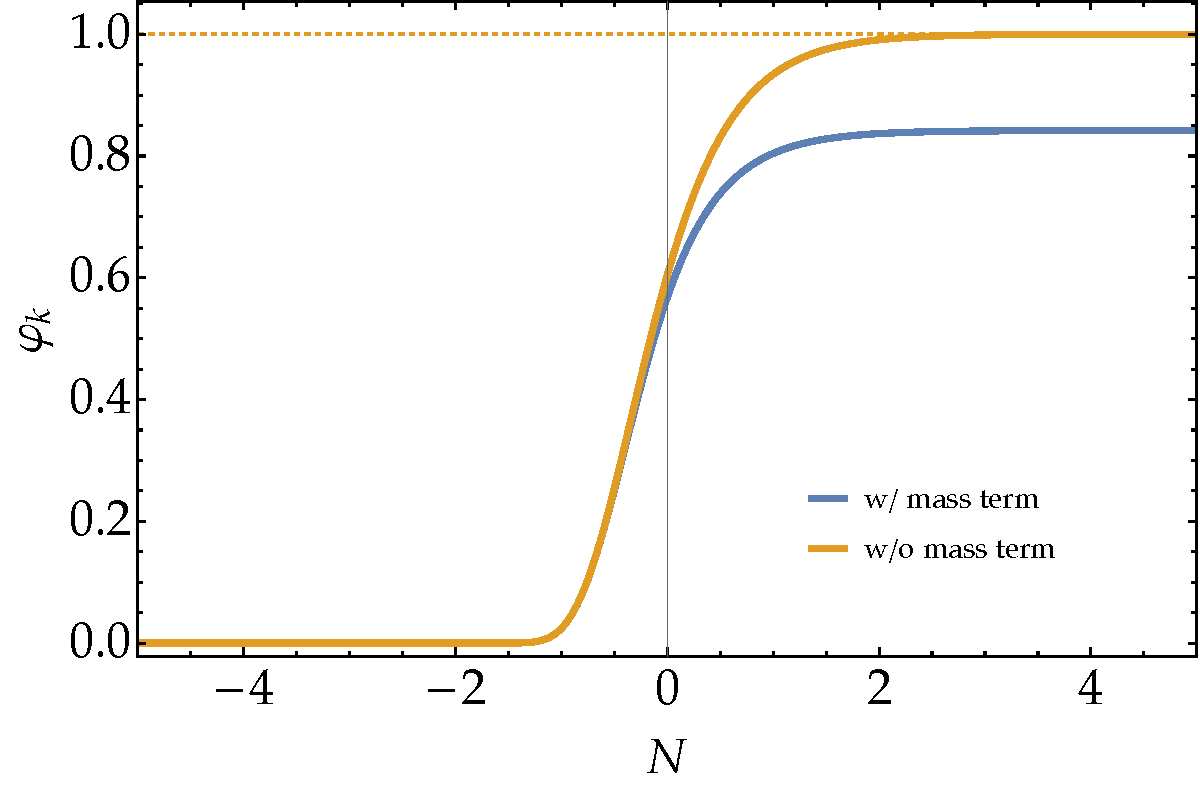
\includegraphics[width=\hsize]{figs/Gaussian.pdf}
		\end{minipage}
		\begin{minipage}{0.5\hsize}
			\centering
			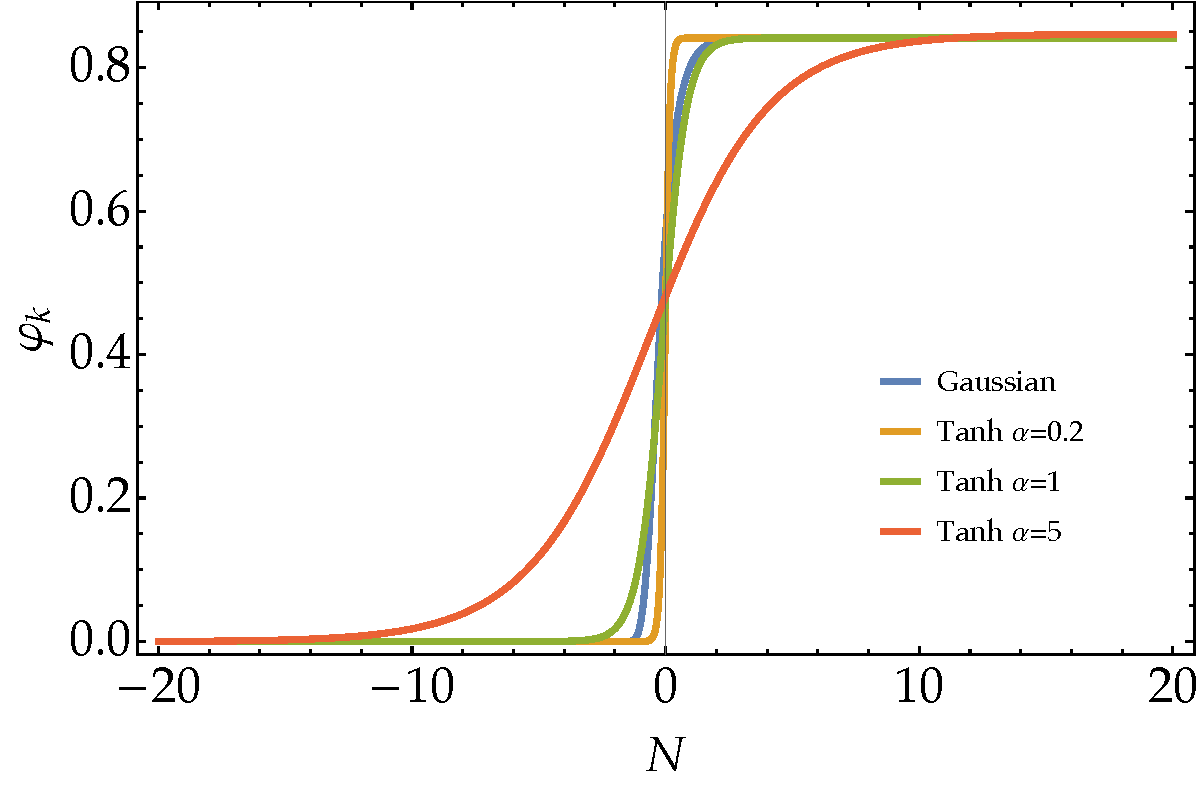
\includegraphics[width=\hsize]{figs/several_window.pdf}
		\end{minipage}
	\end{tabular}
	\caption{}
	\label{fig: phik}
\end{figure}

To see it, we adopt more realistic smooth window function. In this case, the value of the noise term can be assumed to be proportional to
$-\dot{W}_t$ at each time, where its overall coefficient is determined (randomly but a priori) by the variance-$\calP_\phi$ Gaussian.
In the left panel of Fig.~\ref{fig: phik}, we plot the evolution of $\varphi_k$ with or without the mass term where the noise amplitude is normalized
to unity. It shows that the mass term the final amplitude of $\varphi_k$ to around $0.84\times(\text{noise amp.})$.
Also we adopt the hyperbolic tangent window $W_\text{T}=\frac{1}{2}\left(\tanh\left(\frac{\log k-\log k_\sigma}{\alpha}\right)+1\right)$
where $\alpha$ determines the sharpness of its window. In the right panel of Fig.~\ref{fig: phik}, we plot the results for the Gaussian window
and hyperbolic tangent window with several values of $\alpha$. One can see that the final value of $\varphi_k$ hardly depends on the type nor sharpness
of the window function.

From these results, one can conclude the new mass term effectively reduces the noise amplitude by about 0.84 times.
However, at least for the test particle, $\braket{\varphi_k\varphi_{k^\prime}}$ should be consistent with the simple QFT's result 
$\left(\frac{H}{2\pi}\right)^2\delta(\log k-\log k^\prime)$, and such a reduction is quite weird...






\section{Non-canonical multi-field}

The extension to the non-canonical multi-field case which is described by the action
\bae{
	S=\int\dd^4x\sqrt{-g}\left[\frac{\Mpl^2}{2}R-\frac{1}{2}\gamma_{IJ}(\phi)g^{\mu\nu}\partial_\mu\phi^I\partial_\nu\phi^J-V(\phi)\right],
}
is straightforward. The conjugate momentum is given by
\bae{
	\pi_I=\var{S}{\dot{\phi}^I}=\frac{a^3}{N}\gamma_{IJ}(\phi)(\dot{\phi}^I-\beta^i\partial_i\phi^I),
}
and the action can be written as
\bae{
	S=\int\dd^4x(\pi_I\dot{\phi}^I-\mathcal{H}),
}
in terms of the Hamiltonian $\mathcal{H}$:
\bae{
	\mathcal{H}=a^3N_\IR\left(\frac{1}{2a^6}\gamma^{IJ}\pi_I\pi_J+\frac{1}{2a^2}\gamma_{IJ}\partial_i\phi^I\partial_i\phi^J+V
	-\frac{1}{2}\Mpl^2R\right)+\pi_I\beta^i\partial_i\phi^I.
}
Decomposing physical variables into IR and UV parts, the quadratic action in UV modes is given by
\bae{
	S\simeq&S^{(0)}+S^{(1)}+S^{(2)}, \nonumber \\
	S^{(0)}=&\int\dd^4x\left[\varpi_I\dot{\varphi}^I-a^3N_\IR\left(\frac{1}{2a^6}\gamma^{IJ}\varpi_I\varpi_J+V+\frac{3\Mpl^2H^2}{N_\IR^2}\right)\right], \\
	S^{(1)}=&\int\dd^4x\left[P_I\left(\dot{\varphi}^I-\frac{N_\IR}{a^3}\gamma^{IJ}\varpi_J\right)
	-Q^I\left(\dot{\varpi}_I+\frac{N_\IR}{2a^3}\gamma^{JK}{}_{,I}\varpi_J\varpi_K+a^3N_\IR V_I\right) \right. \nonumber \\
	&\left.-a^3\alpha\left(\frac{1}{2a^6}\gamma^{IJ}\varpi_I\varpi_J+V-\frac{3\Mpl^2H^2}{N_\IR^2}\right)\right], \\
	S^{(2)}=&\int\dd^4x\left[-\frac{3\Mpl^2H^2a^3}{N_\IR^3}\alpha^2-a^3\alpha\left(\frac{1}{a^6}\gamma^{IJ}\varpi_IP_J
	+\frac{1}{2a^6}\gamma^{IJ}{}_{,K}Q^K\varpi_I\varpi_J+V_IQ^I+\frac{2\Mpl^2H^2}{N_\IR^2}\frac{\nabla^2}{a^2}\psi\right) \right.\nonumber \\
	&+\varpi_IQ^I\frac{\nabla^2}{a^2}\psi-a^3N_\IR\left(\frac{1}{2a^6}\gamma^{IJ}P_IP_J+\frac{1}{a^6}\gamma^{IJ}{}_{,K}Q^K\varpi_IP_J
	+\frac{1}{4a^6}\gamma^{IJ}{}_{,KL}\varpi_I\varpi_JQ^KQ^L \right. \nonumber \\
	& \left.\left.-\frac{1}{2}\gamma_{IJ}Q^I\frac{\nabla^2}{a^2}Q^J
	+\frac{1}{2}V_{IJ}Q^IQ^J\right)
	+P_I\dot{Q}^I\right].
}
Again the Friedmann equation
\bae{
	\var{S^{(1)}}{\alpha}=0, \quad \Leftrightarrow \quad F:=\frac{1}{2a^6}\gamma^{IJ}\varpi_I\varpi_J+V-\frac{3\Mpl^2H^2}{N_\IR^2}=0,
}
will hold irrespectively of noise.

The momentum constraint $\delta S/\delta\psi=0$ gives
\bae{
	\alpha=\frac{N_\IR^2}{2\Mpl^2H^2a^3}\varpi_IQ^I,
}
which leads to
\bae{
	S^{(0)}&=\int\dd^4x\left[\varpi_I\dot{\varphi}^I-a^3N_\IR\left(\frac{1}{2a^6}\gamma^{IJ}\varpi_I\varpi_J+V+\frac{3\Mpl^2H^2}{N_\IR^2}\right)\right], \\
	S^{(1)}&=\int\dd^4xQ_X^IE_{XI}, \quad\quad S^{(2)}=\int\dd^4x\frac{1}{2}Q_X^I\Lambda_{XYIJ}Q_X^J,
}
with
\bae{
	\bce{
		\dps
		Q_Q^I=Q^I, \quad\quad Q_P^I=P_I, \\[10pt]
		\dps
		E_{QI}=-\left(\dot{\varpi}_I+\frac{N_\IR}{2a^3}\gamma^{JK}{}_{,I}\varpi_J\varpi_K+a^3N_\IR V_I+\frac{N_\IR^2}{2\Mpl^2H}\varpi_IF\right),
		\quad\quad
		E_P^I=\dot{\varphi}^I-\frac{N_\IR}{a^3}\gamma^{IJ}\varpi_{J}, \\[10pt]
		\dps
		\Lambda_{PP}{}^{IJ}=-\frac{N_\IR}{a^3}\gamma^{IJ}, \quad\quad \Lambda_{PQ}{}^I{}_J=-M_{PQ}^2{}^I{}_J+\delta^I_J\partial_t \\[10pt]
		\dps
		\Lambda_{QPI}{}^J=-M_{PQ}^2{}^J{}_I-\delta^J_I\partial_t, \quad\quad 
		\Lambda_{QQIJ}=a^3N_\IR\left(\gamma_{IJ}\frac{\nabla^2}{a^2}-M_{QQIJ}^2\right)\\[10pt]
		\dps
		M_{PQ}^2{}^I{}_J=\frac{N_\IR^2}{2\Mpl^2Ha^6}\gamma^{IK}\varpi_K\varpi_J+\frac{N_\IR}{a^3}\gamma^{IK}{}_{,J}\varpi_K, \\[10pt]
		\dps
		M_{QQIJ}^2=\frac{N_\IR}{2\Mpl^2Ha^9}\gamma^{KL}{}_{,I}\varpi_K\varpi_L\varpi_J
		+\frac{1}{2a^6}\gamma^{KL}{}_{,IJ}\varpi_K\varpi_L+\frac{N_\IR}{\Mpl^2Ha^3}V_I\varpi_J+V_{IJ}+\frac{3}{2\Mpl^2a^6}\varpi_I\varpi_J.
	}
}
Note that the position of $I$ and $J$ is written so as to correspond with $Q$ in the $XY$ notation,
but it is implicitly taken correctly also for $P$-components (e.g. $E_{XI}=(E_P^I,E_{QI})$).

The UV modes follows the EoM
\bae{
	\Lambda_{XYIJ}Q_Y^J=0, \quad\Leftrightarrow\quad \bce{
		\dps
		\dot{Q}^I=\frac{N_\IR}{a^3}\gamma^{IJ}P_J+M_{PQ}^2{}^I{}_JQ^J, \\[10pt]
		\dps
		\dot{P}_I=-M_{PQ}{}^J{}_IP_J+a^3N_\IR\left(\gamma_{IJ}\frac{\nabla^2}{a^2}-M_{QQ}^2{}_{IJ}\right)Q^J,
	}
}
which should be consistent with the well-known formula (\Blue{to be checked})
\bae{
	&\frac{1}{N_\IR^2}\calD_t\calD_tQ^I+\frac{1}{N_\IR^2}\left(3H-\frac{\dot{N}_\IR}{N_\IR}\right)\calD_tQ^I
	-\frac{\nabla^2}{a^2}Q^I \nonumber \\
	&+\left[V^I{}_{;J}-\frac{1}{a^6}R^I{}_{KLJ}\gamma^{KM}\gamma^{LN}\varpi_M\varpi_N
	-\frac{1}{a^3N_\IR\Mpl^2}\calD_t\left(\frac{N_\IR}{a^3H}\gamma^{IK}\varpi_K\varpi_J\right)\right]Q^J=0,
}
with the classical EoM
\bae{
	\bce{
		\dps
		\dot{\varphi}^I\approx\frac{N_\IR}{a^3}\gamma^{IJ}\varpi_{J}, \\[10pt]
		\dps
		\dot{\varpi}_I\approx-\frac{N_\IR}{2a^3}\gamma^{JK}{}_{,I}\varpi_J\varpi_K-a^3N_\IR V_I.
	}
}

Introducing bar indices as
\bae{
	\varphi_{\bar{Q}I}=-\varpi_I, \quad\quad \varphi_{\bar{P}}^I=\varphi^I,
}
and following the same procedure as the single field case, one finds that the influence action is given by
\bae{
	\SIA=&\frac{i}{2}\int\dd^4x\dd^4x^\prime\varphi^\Delta_{\bar{X}I}(x)\Re[\Pi_{XY}{}^{IJ}(x,x^\prime)]\varphi^\Delta_{\bar{Y}J}(x^\prime) \nonumber \\
	&-2\int\dd^4x\dd^4x^\prime\theta(t-t^\prime)\varphi^\Delta_{\bar{X}I}(x)\Im[\Pi_{XY}{}^{IJ}(x,x^\prime)]\bar{\varphi}_{\bar{Y}J}(x^\prime),
}
where
\bae{
	\Pi_{XY}{}^{IJ}(x,x^\prime)=\int\dk\ee^{i\mathbf{k}\cdot(\mathbf{x}-\mathbf{x}^\prime)}\dot{W}_t\dot{W}_{t^\prime}
	\phi_{X\alpha}^I(t,k)\phi_{Y\alpha}^{J*}(t^\prime,k).
}
Here $\phi_{X\alpha}^I(t,k)$ is the mode function defined by
\bae{
	\hat{\phi}_X^I(x)=\int\dk W_t\left[\phi_{X\alpha}^I(t,k)\hat{a}_\alpha(\mathbf{k})\ee^{i\mathbf{k}\cdot\mathbf{x}}
	+\phi_{X\alpha}^{I*}(t,k)\hat{a}^\dagger_\alpha(\mathbf{k})\ee^{i\mathbf{k}\cdot\mathbf{x}}\right],
}
with the annihilation-creation operator
\bae{
	[\hat{a}_\alpha(\mathbf{k}),\hat{a}^\dagger_\beta(\mathbf{k^\prime})]=(2\pi)^3\delta_{\alpha\beta}\delta^{(3)}(\mathbf{k}-\mathbf{k}^\prime).
}
The imaginary part of $\SIA$ gives rise to the noise terms as
\bae{
	\braket{\xi_X^I(x)}=0, \quad\quad \braket{\xi_X^I(x)\xi_Y^J(x^\prime)}=\Re[\Pi_{XY}{}^{IJ}(x,x^\prime)],
}
The real effective action reads
\bae{
	S_\text{eff}=S^{(0),+}-S^{(0),-}+\int\dd^4x\xi_X^I(x)\varphi^\Delta_{\bar{X}I}(x)
	-2\int\dd^4x\dd^4x^\prime\theta(t-t^\prime)\varphi^\Delta_{\bar{X}I}(x)\Im[\Pi_{XY}{}^{IJ}(x,x^\prime)]\bar{\varphi}_{\bar{Y}J}(x^\prime),
}
and the corresponding Langevin equations are
\bae{
	\dot{\varphi}^I=&\frac{N_\IR}{a^3}\gamma^{IJ}\varpi_J+\xi_Q^I \nonumber \\
	&+2\int^t\dd^4x^\prime\Im[\Pi_{QQ}{}^{IJ}(x,x^\prime)]\varpi_J(x^\prime)
	-\int^t\dd^4x^\prime\Im[\Pi_{QP}{}^I{}_J(x,x^\prime)]\varphi^J(x^\prime), \\
	\dot{\varpi}_I=&-\frac{N_\IR}{2a^3}\gamma^{JK}{}_{,I}\varpi_J\varpi_K-a^3N_\IR V_I+\xi_{PI} \nonumber \\
	&+2\int^t\dd^4x^\prime\Im[\Pi_{PQI}{}^J(x,x^\prime)]\varpi_J(x^\prime)-2\int^t\dd^4x^\prime\Im[\Pi_{PPIJ}(x,x^\prime)]\varphi^J(x^\prime), \\
	\frac{3\Mpl^2H^2}{N_\IR^2}=&\frac{1}{2a^6}\gamma^{IJ}\varpi_I\varpi_J+V.
}


\section{Review of the literature}
\begin{itemize}
\item[\cite{Habib:1992ci}] S. Habib \\
The Langevin eq. is derived in terms of the Hamiltonian language in the EoM approach and
the validity of \emph{classicalization assumption} is clarified by studying the Wigner function.

\item[\cite{Vilenkin:1999kd}] A. Vilenkin\\ 
It is discussed that the Ito integral should be used rather then the Stratonovich integral for the definition of noise
from the time reparametrization invariance of the PDF at boundary. (The Ito integral conserves the causality but does not follow the ordinary 
integration law. On the other hand, the Stratonovich integral can be done as an ordinary integration but breaks the causality.)

\item[\cite{Matarrese:2003ye}] S. Matarrese, M. A. Musso, and A. Riotto\\
The Gaussian window is adopted instead of the sharp step function and the effect of the colorness of noise is
investigated. (The dissipation and mass shift are concluded to be negligible...)

\item[\cite{Matacz:1996gk}] A. Matacz \\
The Langevin eq. is derived in the influence functional approach, but the noise and dissipation are assumed to be caused only by interaction terms
like $\phi^4$, neglecting $\varpi\dot{Q}$ and $P\dot{\varphi}$ terms. The corresponding noise amplitude is completely different from the simple QFT's one
and they wrongly concluded that $\lambda$ in quartic chaotic inflation can be as large as $10^{-6}$, 
compared to the conventional prediction $\lambda\sim10^{-12}$.

\item[\cite{Tanaka:1997iy}] T. Tanaka and M. Sakagami \\
criticizes~\cite{Matacz:1996gk}. The noise and dissipation are similarly derived by interaction terms and they find these cause a decoherence of 
the IR mode, but they seem to assume that there is additional noise caused by the horizon exit of the UV mode and therefore 
the conventional result for $\lambda$ is not changed.

\item[\cite{Shandera:2017qkg}] S. Shandera, N. Agarwal, and A. Kamal \\
integrate out the modes which are slightly superhorizon currently and estimate the cosmic variance for near-horizon modes precisely (?).


\end{itemize}




%\acknowledgments





%\appendix

        



\bibliography{bib/textbook,bib/stochastic_deltaN}
\end{document}


















